\documentclass[twoside]{book}

% Packages required by doxygen
\usepackage{calc}
\usepackage{doxygen}
\usepackage{graphicx}
\usepackage[utf8]{inputenc}
\usepackage{makeidx}
\usepackage{multicol}
\usepackage{multirow}
\usepackage{textcomp}
\usepackage[table]{xcolor}

% Font selection
\usepackage[T1]{fontenc}
\usepackage{mathptmx}
\usepackage[scaled=.90]{helvet}
\usepackage{courier}
\usepackage{amssymb}
\usepackage{sectsty}
\renewcommand{\familydefault}{\sfdefault}
\allsectionsfont{%
  \fontseries{bc}\selectfont%
  \color{darkgray}%
}
\renewcommand{\DoxyLabelFont}{%
  \fontseries{bc}\selectfont%
  \color{darkgray}%
}

% Page & text layout
\usepackage{geometry}
\geometry{%
  a4paper,%
  top=2.5cm,%
  bottom=2.5cm,%
  left=2.5cm,%
  right=2.5cm%
}
\tolerance=750
\hfuzz=15pt
\hbadness=750
\setlength{\emergencystretch}{15pt}
\setlength{\parindent}{0cm}
\setlength{\parskip}{0.2cm}
\makeatletter
\renewcommand{\paragraph}{%
  \@startsection{paragraph}{4}{0ex}{-1.0ex}{1.0ex}{%
    \normalfont\normalsize\bfseries\SS@parafont%
  }%
}
\renewcommand{\subparagraph}{%
  \@startsection{subparagraph}{5}{0ex}{-1.0ex}{1.0ex}{%
    \normalfont\normalsize\bfseries\SS@subparafont%
  }%
}
\makeatother

% Headers & footers
\usepackage{fancyhdr}
\pagestyle{fancyplain}
\fancyhead[LE]{\fancyplain{}{\bfseries\thepage}}
\fancyhead[CE]{\fancyplain{}{}}
\fancyhead[RE]{\fancyplain{}{\bfseries\leftmark}}
\fancyhead[LO]{\fancyplain{}{\bfseries\rightmark}}
\fancyhead[CO]{\fancyplain{}{}}
\fancyhead[RO]{\fancyplain{}{\bfseries\thepage}}
\fancyfoot[LE]{\fancyplain{}{}}
\fancyfoot[CE]{\fancyplain{}{}}
\fancyfoot[RE]{\fancyplain{}{\bfseries\scriptsize Generated on Mon Mar 17 2014 16:17:55 for Benchmark by Doxygen }}
\fancyfoot[LO]{\fancyplain{}{\bfseries\scriptsize Generated on Mon Mar 17 2014 16:17:55 for Benchmark by Doxygen }}
\fancyfoot[CO]{\fancyplain{}{}}
\fancyfoot[RO]{\fancyplain{}{}}
\renewcommand{\footrulewidth}{0.4pt}
\renewcommand{\chaptermark}[1]{%
  \markboth{#1}{}%
}
\renewcommand{\sectionmark}[1]{%
  \markright{\thesection\ #1}%
}

% Indices & bibliography
\usepackage{natbib}
\usepackage[titles]{tocloft}
\setcounter{tocdepth}{3}
\setcounter{secnumdepth}{5}
\makeindex

% Hyperlinks (required, but should be loaded last)
\usepackage{ifpdf}
\ifpdf
  \usepackage[pdftex,pagebackref=true]{hyperref}
\else
  \usepackage[ps2pdf,pagebackref=true]{hyperref}
\fi
\hypersetup{%
  colorlinks=true,%
  linkcolor=blue,%
  citecolor=blue,%
  unicode%
}

% Custom commands
\newcommand{\clearemptydoublepage}{%
  \newpage{\pagestyle{empty}\cleardoublepage}%
}


%===== C O N T E N T S =====

\begin{document}

% Titlepage & ToC
\hypersetup{pageanchor=false}
\pagenumbering{roman}
\begin{titlepage}
\vspace*{7cm}
\begin{center}%
{\Large Benchmark \\[1ex]\large 1.\-1.\-a }\\
\vspace*{1cm}
{\large Generated by Doxygen 1.8.4}\\
\vspace*{0.5cm}
{\small Mon Mar 17 2014 16:17:55}\\
\end{center}
\end{titlepage}
\clearemptydoublepage
\tableofcontents
\clearemptydoublepage
\pagenumbering{arabic}
\hypersetup{pageanchor=true}

%--- Begin generated contents ---
\chapter{Benchmark}
\label{index}\hypertarget{index}{}\begin{DoxyAuthor}{Author}
Pawel Zurek 
\end{DoxyAuthor}
\begin{DoxyDate}{Date}
16.\-03.\-2014 
\end{DoxyDate}
\begin{DoxyVersion}{Version}
1.\-1.\-b
\end{DoxyVersion}
Program umożliwia liczenie czasu trwania operacji wypelniania liczbami stosu / kolejki.\hypertarget{index_etykieta-wazne-cechy}{}\section{Najważniejsze cechy}\label{index_etykieta-wazne-cechy}
Program sluzy do liczenia czasu wypelnienia liczbami stosow i kolejek za pomoca \-:\par


\par
-\/$>$ list \par
-\/$>$ tablic ( po przekroczeniu rozmiaru tablicy, rozmiar powiekszany o jeden ) \par
-\/$>$ tablic ( po przekroczeniu rozmiaru tablicy, rozmiar zwiekszany dwukrotnie )\hypertarget{index_etykieta-op-algorytm}{}\section{Opis algorytmu}\label{index_etykieta-op-algorytm}
Algorytm w tym zadaniu to 6 petli \-: \par
-\/$>$ wypelnienie stosu za pomoca listy \par
-\/$>$ wypelnienie kolejki za pomoca listy \par
-\/$>$ wypelnienie stosu za pomoca tablicy ( rozmiar o jeden ) \par
-\/$>$ wypelnienie stosu za pomoca tablicy ( rozmiar x2 ) \par
-\/$>$ wypelnienie kolejki za pomoca tablicy ( rozmiar o jeden ) \par
-\/$>$ wypelnienie kolejki za pomoca tablicy ( rozmiar x2)

\par
,na ktora sklada sie wypelnienie nastepujaca iloscia elementow\-:

\par
-\/$>$ 10 \par
-\/$>$ 100 \par
-\/$>$ 1000 \par
-\/$>$ 10000

Czasy sa wyprowadzane na standartowe wyjscie. 
\chapter{Class Index}
\section{Class List}
Here are the classes, structs, unions and interfaces with brief descriptions\-:\begin{DoxyCompactList}
\item\contentsline{section}{\hyperlink{class_graf}{Graf} \\*Modeluje pojecie graf. Klasa sluzy glownie do wykonania algorytmu wyszukiwania, czyli znalezienia polaczenia miedzy dwoma punktami }{\pageref{class_graf}}{}
\item\contentsline{section}{\hyperlink{structpor}{por} \\*Struktura porownywania Struktura ta ma na celu ulatwienie dzialania algorytmu wyszukiwania ( Dijkstry ) Prownuje ona wartosci drogi miedzy dwoma wezlami }{\pageref{structpor}}{}
\item\contentsline{section}{\hyperlink{struct_wezel}{Wezel} \\*Struktura Wezla Struktura ta ma zdefiniowane dwie zmienne nr oraz g, ktore odpowiadaja za przechowywanie numer wierzcholkana oraz droge jaka juz przebyl od poczatku dzialania wyszukiwania }{\pageref{struct_wezel}}{}
\item\contentsline{section}{\hyperlink{class_wierzcholek}{Wierzcholek} \\*Definicje dla klasy \hyperlink{class_wierzcholek}{Wierzcholek} Struktura ta ma zdefiniowane dwie zmienne sasiad oraz waga. Przy wczytywaniu pliku dodajac wierzcholek dodajemy odrazu informacje o aktualnym sasiedzie oraz o wadze polaczenia miedzy wierzcholkiem i sasiadem }{\pageref{class_wierzcholek}}{}
\end{DoxyCompactList}

\chapter{File Index}
\section{File List}
Here is a list of all files with brief descriptions\-:\begin{DoxyCompactList}
\item\contentsline{section}{/home/pawel/\-Dokumenty/programowanie/pamsi/projekt\-\_\-znajomi/prj/inc/\hyperlink{_dijkstry_8hh}{Dijkstry.\-hh} \\*Definicje funkcji dla klasy graf }{\pageref{_dijkstry_8hh}}{}
\item\contentsline{section}{/home/pawel/\-Dokumenty/programowanie/pamsi/projekt\-\_\-znajomi/prj/src/\hyperlink{_dijkstry_8cpp}{Dijkstry.\-cpp} \\*Plik zawiera funkcje z klasy graf }{\pageref{_dijkstry_8cpp}}{}
\item\contentsline{section}{/home/pawel/\-Dokumenty/programowanie/pamsi/projekt\-\_\-znajomi/prj/src/\hyperlink{main_8cpp}{main.\-cpp} \\*Plik zawiera funkcje \hyperlink{main_8cpp_ae66f6b31b5ad750f1fe042a706a4e3d4}{main()} }{\pageref{main_8cpp}}{}
\end{DoxyCompactList}

\chapter{Class Documentation}
\hypertarget{classbenchmark}{\section{benchmark Class Reference}
\label{classbenchmark}\index{benchmark@{benchmark}}
}


Modeluje pojecie Benchmark.  




{\ttfamily \#include $<$benchmark.\-hh$>$}

\subsection*{Public Member Functions}
\begin{DoxyCompactItemize}
\item 
\hyperlink{classbenchmark_af56f1d9420c5c1ccc65e4f6aac54658d}{benchmark} ()
\begin{DoxyCompactList}\small\item\em Konstruktor klasy Benchmark. \end{DoxyCompactList}\item 
void \hyperlink{classbenchmark_a42ab532c49030406366e859f9b3f29f8}{czas\-\_\-start} ()
\begin{DoxyCompactList}\small\item\em Funkcja pomocnicza mierzenia czasu. \end{DoxyCompactList}\item 
void \hyperlink{classbenchmark_a9beb25d3e65b94c1ac7c085d8105fe65}{czas\-\_\-stop} ()
\begin{DoxyCompactList}\small\item\em Funkcja pomocnicza mierzenia czasu. \end{DoxyCompactList}\item 
double \hyperlink{classbenchmark_a613a8792feca7c2622355922d64d6fcd}{ile\-\_\-czasu} ()
\begin{DoxyCompactList}\small\item\em Funkcja obliczania czasu dzialania programu. \end{DoxyCompactList}\item 
void \hyperlink{classbenchmark_a845da6947383df74d871e273bf225721}{wykonaj\-\_\-algorytn\-\_\-sortowanie} ()
\begin{DoxyCompactList}\small\item\em Funkcja wykonujaca algorytm. \end{DoxyCompactList}\item 
void \hyperlink{classbenchmark_aedc5a477317912eb0d9ca5f9f1da3b7c}{algorytm} ()
\begin{DoxyCompactList}\small\item\em Funkcja wykonujaca algorytm. \end{DoxyCompactList}\item 
void \hyperlink{classbenchmark_a45a6a3fcaf8d09f172f2776451d67c9b}{wyswietl\-\_\-wszystko} (double $\ast$c, double $\ast$q, double $\ast$m, double $\ast$h, int n, int s)
\begin{DoxyCompactList}\small\item\em Funkcja wyswietalnia wynikow. \end{DoxyCompactList}\end{DoxyCompactItemize}
\subsection*{Private Attributes}
\begin{DoxyCompactItemize}
\item 
double \hyperlink{classbenchmark_a90e6eda0144befd3f3bc1a881904fb57}{elapsed\-Time}
\begin{DoxyCompactList}\small\item\em Pole typu double, bedzie uzywane do mierzenia czasu dzialania pojedynczego wypelniania. \end{DoxyCompactList}\item 
double \hyperlink{classbenchmark_a563b747421276232836b7711b6881ec8}{czas}
\begin{DoxyCompactList}\small\item\em Pole typu double, bedzie uzywane do mierzenia calkowitego czasu dzialania programu. \end{DoxyCompactList}\item 
double \hyperlink{classbenchmark_af677300c0b0a0086f306a0a08a6172b9}{czas\-\_\-caly}
\begin{DoxyCompactList}\small\item\em Pole typu double, bedzie uzywane do mierzenia calkowitego czasu dzialania programu. ! \end{DoxyCompactList}\item 
timeval \hyperlink{classbenchmark_a7789217b36df3b3ae427ceaaa2694d0b}{t1}
\begin{DoxyCompactList}\small\item\em Pole typu timeval, pomoc do liczenia czasu dzialania operacji krotkich ( tzn pojedynczego dzialania) \end{DoxyCompactList}\item 
timeval \hyperlink{classbenchmark_aea9f22e585c0c5826329e48a97a99803}{t2}
\end{DoxyCompactItemize}


\subsection{Detailed Description}
Modeluje pojecie Benchmark. 

Klasa sluzy do przeprowadzenia Benchmarku programu, tzn \-: -\/$>$ wczytania dowolnego zestawu danych o ilosci elementow \-: \par
-\/$>$ 10 \par
-\/$>$ 100 \par
-\/$>$ 1000 \par
-\/$>$ 10000 \par
-\/$>$ 100000 \par
-\/$>$ 1000000 \par
 Trzema roznymi metodami \-: \par
 -\/$>$ Quick Sort \par
 -\/$>$ Merge Sort \par
 -\/$>$ Heap Sort \par
 Można jeszcze wybrać ile razy ma zostać wykonany program. \par
-\/$>$ Na koniec zostana wyswietlone czasy kazdej akcji z osobna oraz czas calkowity 

Definition at line 41 of file benchmark.\-hh.



\subsection{Constructor \& Destructor Documentation}
\hypertarget{classbenchmark_af56f1d9420c5c1ccc65e4f6aac54658d}{\index{benchmark@{benchmark}!benchmark@{benchmark}}
\index{benchmark@{benchmark}!benchmark@{benchmark}}
\subsubsection[{benchmark}]{\setlength{\rightskip}{0pt plus 5cm}benchmark\-::benchmark (
\begin{DoxyParamCaption}
{}
\end{DoxyParamCaption}
)\hspace{0.3cm}{\ttfamily [inline]}}}\label{classbenchmark_af56f1d9420c5c1ccc65e4f6aac54658d}


Konstruktor klasy Benchmark. 

Konstruktor jest bezparametryczny, inicjalizuje wszystkie skladowe klasy wartosciami zerowymi. 

Definition at line 71 of file benchmark.\-hh.



\subsection{Member Function Documentation}
\hypertarget{classbenchmark_aedc5a477317912eb0d9ca5f9f1da3b7c}{\index{benchmark@{benchmark}!algorytm@{algorytm}}
\index{algorytm@{algorytm}!benchmark@{benchmark}}
\subsubsection[{algorytm}]{\setlength{\rightskip}{0pt plus 5cm}void benchmark\-::algorytm (
\begin{DoxyParamCaption}
{}
\end{DoxyParamCaption}
)}}\label{classbenchmark_aedc5a477317912eb0d9ca5f9f1da3b7c}


Funkcja wykonujaca algorytm. 

Wykonanie algorytmu ma przebieg \-:\par
 -\/$>$ posortowanie wybranego pliku trzema metodami\-: \par

\begin{DoxyItemize}
\item Quick Sort
\item Merge Sort
\item Heap Sort -\/$>$ po każdym posortowaniu, obiekt jest całkowicie zerowany\par
 -\/$>$ wszystko to wykonuje się zadana przez uzytkownika ilosc razy \par
 
\end{DoxyItemize}

Definition at line 98 of file benchmark.\-cpp.



Here is the call graph for this function\-:\nopagebreak
\begin{figure}[H]
\begin{center}
\leavevmode
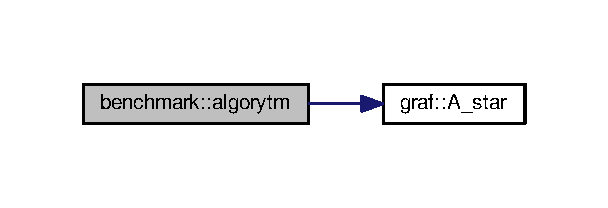
\includegraphics[width=350pt]{classbenchmark_aedc5a477317912eb0d9ca5f9f1da3b7c_cgraph}
\end{center}
\end{figure}




Here is the caller graph for this function\-:\nopagebreak
\begin{figure}[H]
\begin{center}
\leavevmode
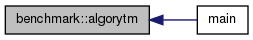
\includegraphics[width=262pt]{classbenchmark_aedc5a477317912eb0d9ca5f9f1da3b7c_icgraph}
\end{center}
\end{figure}


\hypertarget{classbenchmark_a42ab532c49030406366e859f9b3f29f8}{\index{benchmark@{benchmark}!czas\-\_\-start@{czas\-\_\-start}}
\index{czas\-\_\-start@{czas\-\_\-start}!benchmark@{benchmark}}
\subsubsection[{czas\-\_\-start}]{\setlength{\rightskip}{0pt plus 5cm}void benchmark\-::czas\-\_\-start (
\begin{DoxyParamCaption}
{}
\end{DoxyParamCaption}
)}}\label{classbenchmark_a42ab532c49030406366e859f9b3f29f8}


Funkcja pomocnicza mierzenia czasu. 

Funkcja zaczyna liczyc czas od momentu wywolania tej metody Sluzy do liczenia czasu wykonywania pojedynczego wypelniania stosu/kolejki 

Definition at line 14 of file benchmark.\-cpp.

\hypertarget{classbenchmark_a9beb25d3e65b94c1ac7c085d8105fe65}{\index{benchmark@{benchmark}!czas\-\_\-stop@{czas\-\_\-stop}}
\index{czas\-\_\-stop@{czas\-\_\-stop}!benchmark@{benchmark}}
\subsubsection[{czas\-\_\-stop}]{\setlength{\rightskip}{0pt plus 5cm}void benchmark\-::czas\-\_\-stop (
\begin{DoxyParamCaption}
{}
\end{DoxyParamCaption}
)}}\label{classbenchmark_a9beb25d3e65b94c1ac7c085d8105fe65}


Funkcja pomocnicza mierzenia czasu. 

Funkcja konczy liczyc czas od momentu wywolania tej metody Sluzy do liczenia czasu wykonywania pojedynczego wypelniania stosu/kolejki 

Definition at line 17 of file benchmark.\-cpp.

\hypertarget{classbenchmark_a613a8792feca7c2622355922d64d6fcd}{\index{benchmark@{benchmark}!ile\-\_\-czasu@{ile\-\_\-czasu}}
\index{ile\-\_\-czasu@{ile\-\_\-czasu}!benchmark@{benchmark}}
\subsubsection[{ile\-\_\-czasu}]{\setlength{\rightskip}{0pt plus 5cm}double benchmark\-::ile\-\_\-czasu (
\begin{DoxyParamCaption}
{}
\end{DoxyParamCaption}
)}}\label{classbenchmark_a613a8792feca7c2622355922d64d6fcd}


Funkcja obliczania czasu dzialania programu. 

Funkcja podaje czas wykonywania pojedynczego wypelniania stosu/kolejki

\begin{DoxyReturn}{Returns}
elapsed\-Time -\/$>$ zmienna typu double ( wynik obliczen ) 
\end{DoxyReturn}


Definition at line 20 of file benchmark.\-cpp.

\hypertarget{classbenchmark_a845da6947383df74d871e273bf225721}{\index{benchmark@{benchmark}!wykonaj\-\_\-algorytn\-\_\-sortowanie@{wykonaj\-\_\-algorytn\-\_\-sortowanie}}
\index{wykonaj\-\_\-algorytn\-\_\-sortowanie@{wykonaj\-\_\-algorytn\-\_\-sortowanie}!benchmark@{benchmark}}
\subsubsection[{wykonaj\-\_\-algorytn\-\_\-sortowanie}]{\setlength{\rightskip}{0pt plus 5cm}void benchmark\-::wykonaj\-\_\-algorytn\-\_\-sortowanie (
\begin{DoxyParamCaption}
{}
\end{DoxyParamCaption}
)}}\label{classbenchmark_a845da6947383df74d871e273bf225721}


Funkcja wykonujaca algorytm. 

Wykonanie algorytmu ma przebieg \-:\par
 -\/$>$ posortowanie danych metoda Quick Sort\par
 -\/$>$ posortowanie danych metoda Merge Sort\par
 -\/$>$ posortowanie danych metoda Heap Sort\par
 \par
 Dla \-:\par

\begin{DoxyItemize}
\item 10 elementow \par

\item 100 elementow \par

\item 1000 elementow \par

\item 10000 elementow \par

\item 100000 elementow \par

\item 1000000 elementow \par
 
\end{DoxyItemize}

Definition at line 27 of file benchmark.\-cpp.



Here is the call graph for this function\-:\nopagebreak
\begin{figure}[H]
\begin{center}
\leavevmode
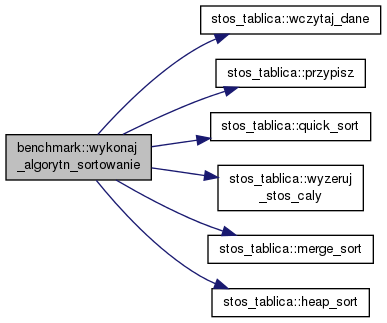
\includegraphics[width=350pt]{classbenchmark_a845da6947383df74d871e273bf225721_cgraph}
\end{center}
\end{figure}


\hypertarget{classbenchmark_a45a6a3fcaf8d09f172f2776451d67c9b}{\index{benchmark@{benchmark}!wyswietl\-\_\-wszystko@{wyswietl\-\_\-wszystko}}
\index{wyswietl\-\_\-wszystko@{wyswietl\-\_\-wszystko}!benchmark@{benchmark}}
\subsubsection[{wyswietl\-\_\-wszystko}]{\setlength{\rightskip}{0pt plus 5cm}void benchmark\-::wyswietl\-\_\-wszystko (
\begin{DoxyParamCaption}
\item[{double $\ast$}]{c, }
\item[{double $\ast$}]{q, }
\item[{double $\ast$}]{m, }
\item[{double $\ast$}]{h, }
\item[{int}]{n, }
\item[{int}]{s}
\end{DoxyParamCaption}
)}}\label{classbenchmark_a45a6a3fcaf8d09f172f2776451d67c9b}


Funkcja wyswietalnia wynikow. 

Funkcja wyswietla wszystkie czasy liczone w programie. Tzn\-: Czasy wszystkich wykonan dla kazdego sortowania, najwolniejsze, najszybsze oraz srednie wykonanie. Dodatkowo czas wykonania calej petli za kazdym razem


\begin{DoxyParams}{Parameters}
{\em c} & -\/$>$ wskaznik na zmienna typu double, przechowuje adres pola czasu calkowitego ( czasy ) \\
\hline
{\em q} & -\/$>$ wskaznik na zmienna typu double, przechowuje adres pola czasu wykonywania Quick Sort ( quick ) \\
\hline
{\em m} & -\/$>$ wskaznik na zmienna typu double, przechowuje adres pola czasu wykonywania Merge Sort ( merge ) \\
\hline
{\em h} & -\/$>$ wskaznik na zmienna typu double, przechowuje adres pola czasu wykonywania Heap Sort ( heap ) \\
\hline
{\em n} & -\/$>$ zmienna typu int, przechowuje adres pola, w ktorym jest informacja o tym ile razy zostal wykonany algorytm ( ile\-\_\-razy ) \\
\hline
{\em s} & -\/$>$ zmienna typu int, przechowuje adres pola rozmiaru tablicy ( size ) \\
\hline
\end{DoxyParams}


Definition at line 149 of file benchmark.\-cpp.



\subsection{Member Data Documentation}
\hypertarget{classbenchmark_a563b747421276232836b7711b6881ec8}{\index{benchmark@{benchmark}!czas@{czas}}
\index{czas@{czas}!benchmark@{benchmark}}
\subsubsection[{czas}]{\setlength{\rightskip}{0pt plus 5cm}double benchmark\-::czas\hspace{0.3cm}{\ttfamily [private]}}}\label{classbenchmark_a563b747421276232836b7711b6881ec8}


Pole typu double, bedzie uzywane do mierzenia calkowitego czasu dzialania programu. 



Definition at line 51 of file benchmark.\-hh.

\hypertarget{classbenchmark_af677300c0b0a0086f306a0a08a6172b9}{\index{benchmark@{benchmark}!czas\-\_\-caly@{czas\-\_\-caly}}
\index{czas\-\_\-caly@{czas\-\_\-caly}!benchmark@{benchmark}}
\subsubsection[{czas\-\_\-caly}]{\setlength{\rightskip}{0pt plus 5cm}double benchmark\-::czas\-\_\-caly\hspace{0.3cm}{\ttfamily [private]}}}\label{classbenchmark_af677300c0b0a0086f306a0a08a6172b9}


Pole typu double, bedzie uzywane do mierzenia calkowitego czasu dzialania programu. ! 



Definition at line 55 of file benchmark.\-hh.

\hypertarget{classbenchmark_a90e6eda0144befd3f3bc1a881904fb57}{\index{benchmark@{benchmark}!elapsed\-Time@{elapsed\-Time}}
\index{elapsed\-Time@{elapsed\-Time}!benchmark@{benchmark}}
\subsubsection[{elapsed\-Time}]{\setlength{\rightskip}{0pt plus 5cm}double benchmark\-::elapsed\-Time\hspace{0.3cm}{\ttfamily [private]}}}\label{classbenchmark_a90e6eda0144befd3f3bc1a881904fb57}


Pole typu double, bedzie uzywane do mierzenia czasu dzialania pojedynczego wypelniania. 



Definition at line 47 of file benchmark.\-hh.

\hypertarget{classbenchmark_a7789217b36df3b3ae427ceaaa2694d0b}{\index{benchmark@{benchmark}!t1@{t1}}
\index{t1@{t1}!benchmark@{benchmark}}
\subsubsection[{t1}]{\setlength{\rightskip}{0pt plus 5cm}timeval benchmark\-::t1\hspace{0.3cm}{\ttfamily [private]}}}\label{classbenchmark_a7789217b36df3b3ae427ceaaa2694d0b}


Pole typu timeval, pomoc do liczenia czasu dzialania operacji krotkich ( tzn pojedynczego dzialania) 



Definition at line 59 of file benchmark.\-hh.

\hypertarget{classbenchmark_aea9f22e585c0c5826329e48a97a99803}{\index{benchmark@{benchmark}!t2@{t2}}
\index{t2@{t2}!benchmark@{benchmark}}
\subsubsection[{t2}]{\setlength{\rightskip}{0pt plus 5cm}timeval benchmark\-::t2\hspace{0.3cm}{\ttfamily [private]}}}\label{classbenchmark_aea9f22e585c0c5826329e48a97a99803}


Definition at line 59 of file benchmark.\-hh.



The documentation for this class was generated from the following files\-:\begin{DoxyCompactItemize}
\item 
/home/pawel/\-Dokumenty/programowanie/pamsi/sortowaniev2/prj/inc/\hyperlink{benchmark_8hh}{benchmark.\-hh}\item 
/home/pawel/\-Dokumenty/programowanie/pamsi/sortowaniev2/prj/src/\hyperlink{benchmark_8cpp}{benchmark.\-cpp}\end{DoxyCompactItemize}

\hypertarget{classelement}{\section{element Class Reference}
\label{classelement}\index{element@{element}}
}


Modeluje pojecie element.  




{\ttfamily \#include $<$stos\-\_\-lista.\-hh$>$}



Collaboration diagram for element\-:\nopagebreak
\begin{figure}[H]
\begin{center}
\leavevmode
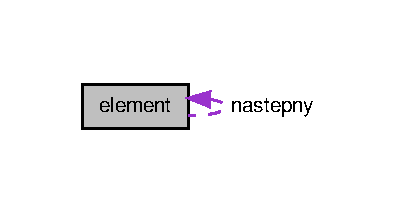
\includegraphics[width=191pt]{classelement__coll__graph}
\end{center}
\end{figure}
\subsection*{Public Attributes}
\begin{DoxyCompactItemize}
\item 
\hyperlink{classelement}{element} $\ast$ \hyperlink{classelement_ab6df52b0e5cfa7c4998a2ab74a8ef53e}{nastepny}
\begin{DoxyCompactList}\small\item\em Pole typu element$\ast$, wskaznik uzywany do laczenia elementow miedzy soba w stos. \end{DoxyCompactList}\item 
int \hyperlink{classelement_a112279ccab2f4e22485125be5bda7b75}{klucz}
\begin{DoxyCompactList}\small\item\em Pole typu int, przechowuje informacje o wartosci danego elementu. \end{DoxyCompactList}\end{DoxyCompactItemize}


\subsection{Detailed Description}
Modeluje pojecie element. 

Element jest klasa,ktora bedzie wpisywana do stosu Klasa ta zawiera informacje o danej wartosci elementu ( klucz ) oraz wskaznik na nastepny element. 

Definition at line 29 of file stos\-\_\-lista.\-hh.



\subsection{Member Data Documentation}
\hypertarget{classelement_a112279ccab2f4e22485125be5bda7b75}{\index{element@{element}!klucz@{klucz}}
\index{klucz@{klucz}!element@{element}}
\subsubsection[{klucz}]{\setlength{\rightskip}{0pt plus 5cm}int element\-::klucz}}\label{classelement_a112279ccab2f4e22485125be5bda7b75}


Pole typu int, przechowuje informacje o wartosci danego elementu. 



Definition at line 39 of file stos\-\_\-lista.\-hh.

\hypertarget{classelement_ab6df52b0e5cfa7c4998a2ab74a8ef53e}{\index{element@{element}!nastepny@{nastepny}}
\index{nastepny@{nastepny}!element@{element}}
\subsubsection[{nastepny}]{\setlength{\rightskip}{0pt plus 5cm}{\bf element}$\ast$ element\-::nastepny}}\label{classelement_ab6df52b0e5cfa7c4998a2ab74a8ef53e}


Pole typu element$\ast$, wskaznik uzywany do laczenia elementow miedzy soba w stos. 



Definition at line 35 of file stos\-\_\-lista.\-hh.



The documentation for this class was generated from the following file\-:\begin{DoxyCompactItemize}
\item 
/home/pawel/\-Dokumenty/programowanie/pamsi/zad3/prj/inc/\hyperlink{stos__lista_8hh}{stos\-\_\-lista.\-hh}\end{DoxyCompactItemize}

\hypertarget{classelementk}{\section{elementk Class Reference}
\label{classelementk}\index{elementk@{elementk}}
}


Modeluje pojecie elementk (zmieniona nazwa, poniewaz \hyperlink{classstos__lista}{stos\-\_\-lista} tez ma klase o nazwie element).  




{\ttfamily \#include $<$kolejka\-\_\-lista.\-hh$>$}



Collaboration diagram for elementk\-:\nopagebreak
\begin{figure}[H]
\begin{center}
\leavevmode
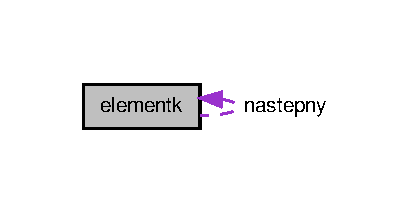
\includegraphics[width=197pt]{classelementk__coll__graph}
\end{center}
\end{figure}
\subsection*{Public Attributes}
\begin{DoxyCompactItemize}
\item 
\hyperlink{classelementk}{elementk} $\ast$ \hyperlink{classelementk_a651594e4ecff4a674b7df913b68b1d55}{nastepny}
\begin{DoxyCompactList}\small\item\em Pole typu element$\ast$, wskaznik uzywany do laczenia elementow miedzy soba w stos. \end{DoxyCompactList}\item 
int \hyperlink{classelementk_a80de941ecbf60bd5189d1c1005c68203}{klucz}
\begin{DoxyCompactList}\small\item\em Pole typu int, przechowuje informacje o wartosci danego elementu. \end{DoxyCompactList}\end{DoxyCompactItemize}


\subsection{Detailed Description}
Modeluje pojecie elementk (zmieniona nazwa, poniewaz \hyperlink{classstos__lista}{stos\-\_\-lista} tez ma klase o nazwie element). 

Element jest klasa,ktora bedzie wpisywana do stosu Klasa ta zawiera informacje o danej wartosci elementu ( klucz ) oraz wskaznik na nastepny element. 

Definition at line 30 of file kolejka\-\_\-lista.\-hh.



\subsection{Member Data Documentation}
\hypertarget{classelementk_a80de941ecbf60bd5189d1c1005c68203}{\index{elementk@{elementk}!klucz@{klucz}}
\index{klucz@{klucz}!elementk@{elementk}}
\subsubsection[{klucz}]{\setlength{\rightskip}{0pt plus 5cm}int elementk\-::klucz}}\label{classelementk_a80de941ecbf60bd5189d1c1005c68203}


Pole typu int, przechowuje informacje o wartosci danego elementu. 



Definition at line 40 of file kolejka\-\_\-lista.\-hh.

\hypertarget{classelementk_a651594e4ecff4a674b7df913b68b1d55}{\index{elementk@{elementk}!nastepny@{nastepny}}
\index{nastepny@{nastepny}!elementk@{elementk}}
\subsubsection[{nastepny}]{\setlength{\rightskip}{0pt plus 5cm}{\bf elementk}$\ast$ elementk\-::nastepny}}\label{classelementk_a651594e4ecff4a674b7df913b68b1d55}


Pole typu element$\ast$, wskaznik uzywany do laczenia elementow miedzy soba w stos. 



Definition at line 36 of file kolejka\-\_\-lista.\-hh.



The documentation for this class was generated from the following file\-:\begin{DoxyCompactItemize}
\item 
/home/pawel/\-Dokumenty/programowanie/pamsi/zad3/prj/inc/\hyperlink{kolejka__lista_8hh}{kolejka\-\_\-lista.\-hh}\end{DoxyCompactItemize}

\hypertarget{classkolejka__lista}{\section{kolejka\-\_\-lista Class Reference}
\label{classkolejka__lista}\index{kolejka\-\_\-lista@{kolejka\-\_\-lista}}
}


Modeluje pojecie Kolejka.  




{\ttfamily \#include $<$kolejka\-\_\-lista.\-hh$>$}



Collaboration diagram for kolejka\-\_\-lista\-:\nopagebreak
\begin{figure}[H]
\begin{center}
\leavevmode
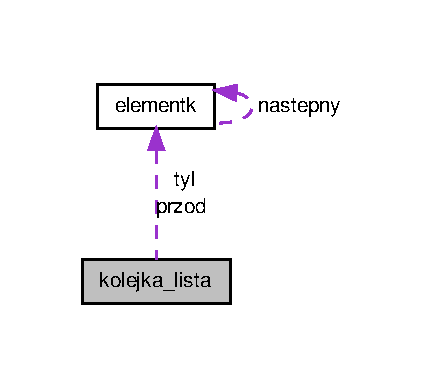
\includegraphics[width=204pt]{classkolejka__lista__coll__graph}
\end{center}
\end{figure}
\subsection*{Public Member Functions}
\begin{DoxyCompactItemize}
\item 
\hyperlink{classkolejka__lista_a501a2eeb46cc914d6aa84e0eab0f7b20}{kolejka\-\_\-lista} ()
\begin{DoxyCompactList}\small\item\em Konstruktor klasy kolejka. \end{DoxyCompactList}\item 
\hyperlink{classkolejka__lista_a01a293936690fd9af18220939a8a934c}{$\sim$kolejka\-\_\-lista} ()
\begin{DoxyCompactList}\small\item\em Destruktor klasy Kolejka. \end{DoxyCompactList}\item 
void \hyperlink{classkolejka__lista_a6b3e5198fc3f572417e718c5c263c184}{wczytaj\-\_\-dane} ()
\begin{DoxyCompactList}\small\item\em Funkcja wczytywania. \end{DoxyCompactList}\item 
void \hyperlink{classkolejka__lista_a0db9fa402ebbd0a4038950d3abddba8c}{wczytaj\-\_\-dane} (string nazwa)
\begin{DoxyCompactList}\small\item\em Funkcja wczytywania. \end{DoxyCompactList}\item 
void \hyperlink{classkolejka__lista_a42a5b9ed3da1c9d3b855999b890ccee3}{pokaz\-\_\-elementy} ()
\begin{DoxyCompactList}\small\item\em Funkcja wyswietlajaca. \end{DoxyCompactList}\item 
bool \hyperlink{classkolejka__lista_a139de3d0627c47ed921d95bd3bc41bae}{isempty} ()
\begin{DoxyCompactList}\small\item\em Funkcja sprawdzania pustosci kolejki. \end{DoxyCompactList}\item 
unsigned \hyperlink{classkolejka__lista_a874481fb9b5c8324205b30c28a58d713}{size} ()
\begin{DoxyCompactList}\small\item\em Funkcja sprawdzania rozmiar kolejki. \end{DoxyCompactList}\item 
\hyperlink{classelementk}{elementk} $\ast$ \hyperlink{classkolejka__lista_abb6cd9a2a527bcaa2515e62c9c6e6813}{push} (\hyperlink{classelementk}{elementk} $\ast$p)
\begin{DoxyCompactList}\small\item\em Funkcja dodajaca element. \end{DoxyCompactList}\item 
void \hyperlink{classkolejka__lista_af92f6af53ded24a2b86c85790797b356}{dodaj\-\_\-element} (int a)
\begin{DoxyCompactList}\small\item\em Funkcja dodajaca element. \end{DoxyCompactList}\item 
\hyperlink{classelementk}{elementk} $\ast$ \hyperlink{classkolejka__lista_a36a5b9c7c4e57e23aa8d2bb9afb223ef}{pop} ()
\begin{DoxyCompactList}\small\item\em Funkcja usuwajaca ostatni element ze stosu. \end{DoxyCompactList}\end{DoxyCompactItemize}
\subsection*{Private Attributes}
\begin{DoxyCompactItemize}
\item 
\hyperlink{classelementk}{elementk} $\ast$ \hyperlink{classkolejka__lista_aedc7846eba7725b49c3de16fa18ae33a}{przod}
\begin{DoxyCompactList}\small\item\em Pole typu element, wskazuje na pierwszy element listy. \end{DoxyCompactList}\item 
\hyperlink{classelementk}{elementk} $\ast$ \hyperlink{classkolejka__lista_a9675dc97e4a026b1556699024e24636e}{tyl}
\begin{DoxyCompactList}\small\item\em Pole typu element, wskazuje na ostatni element listy. \end{DoxyCompactList}\item 
unsigned \hyperlink{classkolejka__lista_a6b12b09e2f057761ac4d5ac1b1c82115}{licznik}
\begin{DoxyCompactList}\small\item\em Pole typu int, bedzie uzywane jako rozmiar kolejki. \end{DoxyCompactList}\end{DoxyCompactItemize}


\subsection{Detailed Description}
Modeluje pojecie Kolejka. 

Stos jest klasa zawierajaca dynamicznie zaalokowane liste 

Definition at line 52 of file kolejka\-\_\-lista.\-hh.



\subsection{Constructor \& Destructor Documentation}
\hypertarget{classkolejka__lista_a501a2eeb46cc914d6aa84e0eab0f7b20}{\index{kolejka\-\_\-lista@{kolejka\-\_\-lista}!kolejka\-\_\-lista@{kolejka\-\_\-lista}}
\index{kolejka\-\_\-lista@{kolejka\-\_\-lista}!kolejka_lista@{kolejka\-\_\-lista}}
\subsubsection[{kolejka\-\_\-lista}]{\setlength{\rightskip}{0pt plus 5cm}kolejka\-\_\-lista\-::kolejka\-\_\-lista (
\begin{DoxyParamCaption}
{}
\end{DoxyParamCaption}
)\hspace{0.3cm}{\ttfamily [inline]}}}\label{classkolejka__lista_a501a2eeb46cc914d6aa84e0eab0f7b20}


Konstruktor klasy kolejka. 

Konstruktor jest bezparametryczny, inicjalizuje wszystkie skladowe klasy wartosciami zerowymi. 

Definition at line 78 of file kolejka\-\_\-lista.\-hh.

\hypertarget{classkolejka__lista_a01a293936690fd9af18220939a8a934c}{\index{kolejka\-\_\-lista@{kolejka\-\_\-lista}!$\sim$kolejka\-\_\-lista@{$\sim$kolejka\-\_\-lista}}
\index{$\sim$kolejka\-\_\-lista@{$\sim$kolejka\-\_\-lista}!kolejka_lista@{kolejka\-\_\-lista}}
\subsubsection[{$\sim$kolejka\-\_\-lista}]{\setlength{\rightskip}{0pt plus 5cm}kolejka\-\_\-lista\-::$\sim$kolejka\-\_\-lista (
\begin{DoxyParamCaption}
{}
\end{DoxyParamCaption}
)\hspace{0.3cm}{\ttfamily [inline]}}}\label{classkolejka__lista_a01a293936690fd9af18220939a8a934c}


Destruktor klasy Kolejka. 

Usuwa dynamicznie zaalokawana liste 

Definition at line 85 of file kolejka\-\_\-lista.\-hh.



\subsection{Member Function Documentation}
\hypertarget{classkolejka__lista_af92f6af53ded24a2b86c85790797b356}{\index{kolejka\-\_\-lista@{kolejka\-\_\-lista}!dodaj\-\_\-element@{dodaj\-\_\-element}}
\index{dodaj\-\_\-element@{dodaj\-\_\-element}!kolejka_lista@{kolejka\-\_\-lista}}
\subsubsection[{dodaj\-\_\-element}]{\setlength{\rightskip}{0pt plus 5cm}void kolejka\-\_\-lista\-::dodaj\-\_\-element (
\begin{DoxyParamCaption}
\item[{int}]{a}
\end{DoxyParamCaption}
)}}\label{classkolejka__lista_af92f6af53ded24a2b86c85790797b356}


Funkcja dodajaca element. 

Funkcja dodaje do stosu element podany przez uzytkownika poprzez wywolanie funkcji \hyperlink{classkolejka__lista_abb6cd9a2a527bcaa2515e62c9c6e6813}{push()}. 
\begin{DoxyParams}{Parameters}
{\em a} & -\/ pole typu int przechowuje wartosc jaka ma byc wpisana \\
\hline
\end{DoxyParams}


Definition at line 61 of file kolejka\-\_\-lista.\-cpp.



Here is the call graph for this function\-:\nopagebreak
\begin{figure}[H]
\begin{center}
\leavevmode
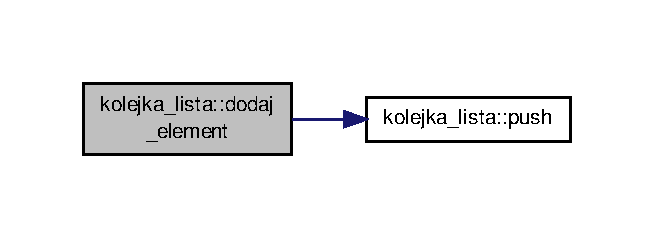
\includegraphics[width=314pt]{classkolejka__lista_af92f6af53ded24a2b86c85790797b356_cgraph}
\end{center}
\end{figure}




Here is the caller graph for this function\-:\nopagebreak
\begin{figure}[H]
\begin{center}
\leavevmode
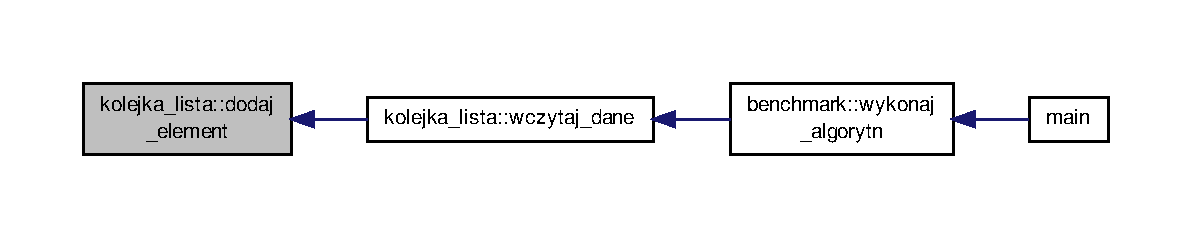
\includegraphics[width=350pt]{classkolejka__lista_af92f6af53ded24a2b86c85790797b356_icgraph}
\end{center}
\end{figure}


\hypertarget{classkolejka__lista_a139de3d0627c47ed921d95bd3bc41bae}{\index{kolejka\-\_\-lista@{kolejka\-\_\-lista}!isempty@{isempty}}
\index{isempty@{isempty}!kolejka_lista@{kolejka\-\_\-lista}}
\subsubsection[{isempty}]{\setlength{\rightskip}{0pt plus 5cm}bool kolejka\-\_\-lista\-::isempty (
\begin{DoxyParamCaption}
{}
\end{DoxyParamCaption}
)}}\label{classkolejka__lista_a139de3d0627c47ed921d95bd3bc41bae}


Funkcja sprawdzania pustosci kolejki. 

Funkcja sprawdza czy kolejka jest pusty

\begin{DoxyReturn}{Returns}
1 -\/$>$ Kolejka pusta 0 -\/$>$ kolejka nie pusta 
\end{DoxyReturn}


Definition at line 6 of file kolejka\-\_\-lista.\-cpp.

\hypertarget{classkolejka__lista_a42a5b9ed3da1c9d3b855999b890ccee3}{\index{kolejka\-\_\-lista@{kolejka\-\_\-lista}!pokaz\-\_\-elementy@{pokaz\-\_\-elementy}}
\index{pokaz\-\_\-elementy@{pokaz\-\_\-elementy}!kolejka_lista@{kolejka\-\_\-lista}}
\subsubsection[{pokaz\-\_\-elementy}]{\setlength{\rightskip}{0pt plus 5cm}void kolejka\-\_\-lista\-::pokaz\-\_\-elementy (
\begin{DoxyParamCaption}
{}
\end{DoxyParamCaption}
)}}\label{classkolejka__lista_a42a5b9ed3da1c9d3b855999b890ccee3}


Funkcja wyswietlajaca. 

Funkcja wyswietla aktualny stan kolejki 

Definition at line 44 of file kolejka\-\_\-lista.\-cpp.

\hypertarget{classkolejka__lista_a36a5b9c7c4e57e23aa8d2bb9afb223ef}{\index{kolejka\-\_\-lista@{kolejka\-\_\-lista}!pop@{pop}}
\index{pop@{pop}!kolejka_lista@{kolejka\-\_\-lista}}
\subsubsection[{pop}]{\setlength{\rightskip}{0pt plus 5cm}{\bf elementk} $\ast$ kolejka\-\_\-lista\-::pop (
\begin{DoxyParamCaption}
{}
\end{DoxyParamCaption}
)}}\label{classkolejka__lista_a36a5b9c7c4e57e23aa8d2bb9afb223ef}


Funkcja usuwajaca ostatni element ze stosu. 

Funkcja usuwa z listy ostatni element i zwraca jego adres.

Jeśli lista jest pusta, to pole tyl zawiera N\-U\-L\-L. W takim przypadku zwracamy N\-U\-L\-L i kończymy.

W przeciwnym razie zapamiętujemy adres ostatniego elementu listy w p. Jeśli lista zawiera tylko jeden element , to pola przod i tyl zawierają ten sam adres. W takim przypadku lista staje się pusta po odłączeniu ostatniego elementu, dlatego wpisujemy w nie adres pusty N\-U\-L\-L.

Jeśli lista zawiera więcej niż jeden element, to przechodzimy kolejno przez wszystkie elementy listy ustawiając pole tyl na adres poprzednika ostatniego elementu. W poprzedniku zerujemy następnik.

Zmniejszamy licznik i zwracamy zapamiętany w p adres ostatniego elementu. 

Definition at line 28 of file kolejka\-\_\-lista.\-cpp.

\hypertarget{classkolejka__lista_abb6cd9a2a527bcaa2515e62c9c6e6813}{\index{kolejka\-\_\-lista@{kolejka\-\_\-lista}!push@{push}}
\index{push@{push}!kolejka_lista@{kolejka\-\_\-lista}}
\subsubsection[{push}]{\setlength{\rightskip}{0pt plus 5cm}{\bf elementk} $\ast$ kolejka\-\_\-lista\-::push (
\begin{DoxyParamCaption}
\item[{{\bf elementk} $\ast$}]{p}
\end{DoxyParamCaption}
)}}\label{classkolejka__lista_abb6cd9a2a527bcaa2515e62c9c6e6813}


Funkcja dodajaca element. 

Funkcja wstawia nowy element p na koniec kolejki i zwraca jego adres.

Jeśli lista zawiera jakieś elementy, to tyl zawsze wskazuje ostatni element listy. W pole nastepny ostatniego elementu wpisujemy w takim przypadku adres wstawianego elementu. W efekcie zostanie on dołączony do końca listy. W polu nastepny nowego elementu umieszczamy adres zerowy N\-U\-L\-L, ponieważ jest on teraz ostatnim elementem i nie posiada następnika.

Lista mogła być pusta. W takim przypadku wstawiony element jest jednocześnie pierwszym i ostatnim. Dlatego do pola przod wpisujemy adres pobrany z pola tyl.

Po wstawieniu elementu zwiększamy licznik licznik i zwracamy adres końca kolejki.


\begin{DoxyParams}{Parameters}
{\em p} & -\/ pole typu element przechowuje wartosc jaka ma byc wpisana \\
\hline
\end{DoxyParams}
\begin{DoxyReturn}{Returns}
adres nowego elementu. 
\end{DoxyReturn}


Definition at line 19 of file kolejka\-\_\-lista.\-cpp.



Here is the caller graph for this function\-:\nopagebreak
\begin{figure}[H]
\begin{center}
\leavevmode
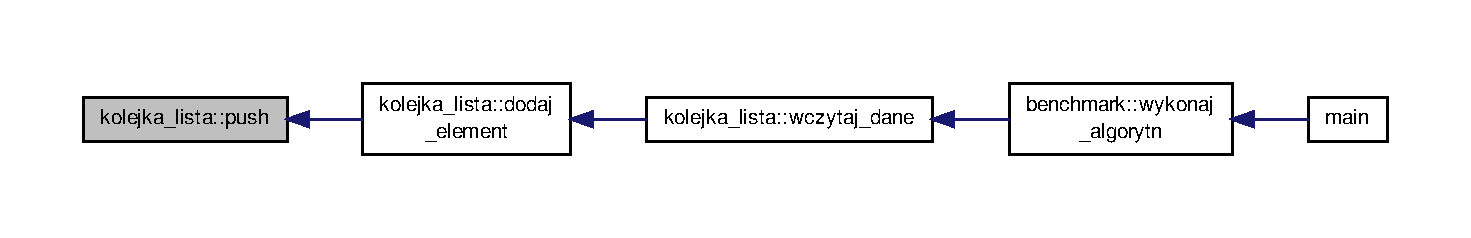
\includegraphics[width=350pt]{classkolejka__lista_abb6cd9a2a527bcaa2515e62c9c6e6813_icgraph}
\end{center}
\end{figure}


\hypertarget{classkolejka__lista_a874481fb9b5c8324205b30c28a58d713}{\index{kolejka\-\_\-lista@{kolejka\-\_\-lista}!size@{size}}
\index{size@{size}!kolejka_lista@{kolejka\-\_\-lista}}
\subsubsection[{size}]{\setlength{\rightskip}{0pt plus 5cm}unsigned kolejka\-\_\-lista\-::size (
\begin{DoxyParamCaption}
{}
\end{DoxyParamCaption}
)}}\label{classkolejka__lista_a874481fb9b5c8324205b30c28a58d713}


Funkcja sprawdzania rozmiar kolejki. 

Funkcja podaje aktualny rozmiar kolejki

\begin{DoxyReturn}{Returns}
rozmiar -\/$>$ rozmiar kolejki 
\end{DoxyReturn}


Definition at line 14 of file kolejka\-\_\-lista.\-cpp.

\hypertarget{classkolejka__lista_a6b3e5198fc3f572417e718c5c263c184}{\index{kolejka\-\_\-lista@{kolejka\-\_\-lista}!wczytaj\-\_\-dane@{wczytaj\-\_\-dane}}
\index{wczytaj\-\_\-dane@{wczytaj\-\_\-dane}!kolejka_lista@{kolejka\-\_\-lista}}
\subsubsection[{wczytaj\-\_\-dane}]{\setlength{\rightskip}{0pt plus 5cm}void kolejka\-\_\-lista\-::wczytaj\-\_\-dane (
\begin{DoxyParamCaption}
{}
\end{DoxyParamCaption}
)}}\label{classkolejka__lista_a6b3e5198fc3f572417e718c5c263c184}


Funkcja wczytywania. 

Funkcja wczytuje wartosci do stosu z podanego pliku przez uzytkownika. 

Definition at line 68 of file kolejka\-\_\-lista.\-cpp.



Here is the call graph for this function\-:\nopagebreak
\begin{figure}[H]
\begin{center}
\leavevmode
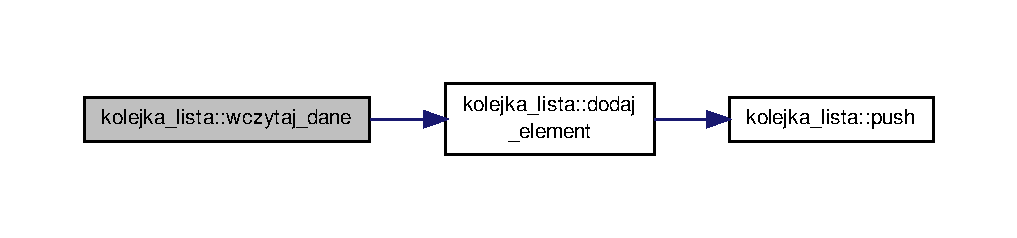
\includegraphics[width=350pt]{classkolejka__lista_a6b3e5198fc3f572417e718c5c263c184_cgraph}
\end{center}
\end{figure}




Here is the caller graph for this function\-:\nopagebreak
\begin{figure}[H]
\begin{center}
\leavevmode
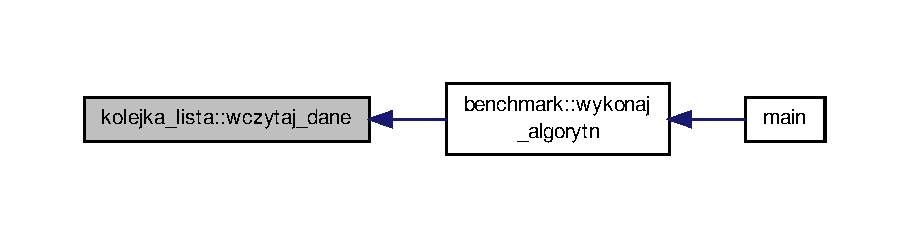
\includegraphics[width=350pt]{classkolejka__lista_a6b3e5198fc3f572417e718c5c263c184_icgraph}
\end{center}
\end{figure}


\hypertarget{classkolejka__lista_a0db9fa402ebbd0a4038950d3abddba8c}{\index{kolejka\-\_\-lista@{kolejka\-\_\-lista}!wczytaj\-\_\-dane@{wczytaj\-\_\-dane}}
\index{wczytaj\-\_\-dane@{wczytaj\-\_\-dane}!kolejka_lista@{kolejka\-\_\-lista}}
\subsubsection[{wczytaj\-\_\-dane}]{\setlength{\rightskip}{0pt plus 5cm}void kolejka\-\_\-lista\-::wczytaj\-\_\-dane (
\begin{DoxyParamCaption}
\item[{string}]{nazwa}
\end{DoxyParamCaption}
)}}\label{classkolejka__lista_a0db9fa402ebbd0a4038950d3abddba8c}


Funkcja wczytywania. 

Funkcja wczytuje wartosci do tabeli po przez wpisanie nazwy jako argument metody Wykorzystuje metode push jako funkcje wpisujaca do kolejki


\begin{DoxyParams}{Parameters}
{\em nazwa} & -\/$>$ zmienna typu string, przechowuje nazwe otwieranego pliku \\
\hline
\end{DoxyParams}


Definition at line 85 of file kolejka\-\_\-lista.\-cpp.



Here is the call graph for this function\-:\nopagebreak
\begin{figure}[H]
\begin{center}
\leavevmode
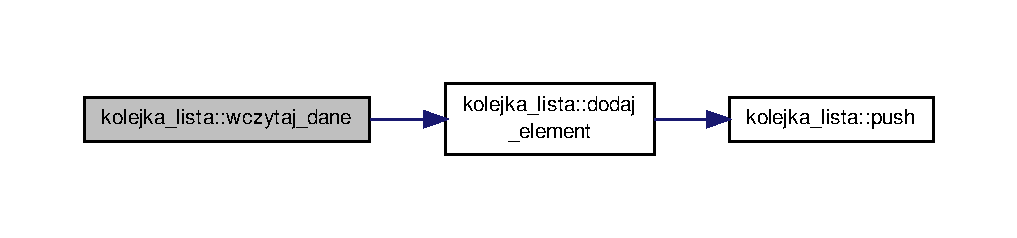
\includegraphics[width=350pt]{classkolejka__lista_a0db9fa402ebbd0a4038950d3abddba8c_cgraph}
\end{center}
\end{figure}




\subsection{Member Data Documentation}
\hypertarget{classkolejka__lista_a6b12b09e2f057761ac4d5ac1b1c82115}{\index{kolejka\-\_\-lista@{kolejka\-\_\-lista}!licznik@{licznik}}
\index{licznik@{licznik}!kolejka_lista@{kolejka\-\_\-lista}}
\subsubsection[{licznik}]{\setlength{\rightskip}{0pt plus 5cm}unsigned kolejka\-\_\-lista\-::licznik\hspace{0.3cm}{\ttfamily [private]}}}\label{classkolejka__lista_a6b12b09e2f057761ac4d5ac1b1c82115}


Pole typu int, bedzie uzywane jako rozmiar kolejki. 



Definition at line 67 of file kolejka\-\_\-lista.\-hh.

\hypertarget{classkolejka__lista_aedc7846eba7725b49c3de16fa18ae33a}{\index{kolejka\-\_\-lista@{kolejka\-\_\-lista}!przod@{przod}}
\index{przod@{przod}!kolejka_lista@{kolejka\-\_\-lista}}
\subsubsection[{przod}]{\setlength{\rightskip}{0pt plus 5cm}{\bf elementk}$\ast$ kolejka\-\_\-lista\-::przod\hspace{0.3cm}{\ttfamily [private]}}}\label{classkolejka__lista_aedc7846eba7725b49c3de16fa18ae33a}


Pole typu element, wskazuje na pierwszy element listy. 



Definition at line 58 of file kolejka\-\_\-lista.\-hh.

\hypertarget{classkolejka__lista_a9675dc97e4a026b1556699024e24636e}{\index{kolejka\-\_\-lista@{kolejka\-\_\-lista}!tyl@{tyl}}
\index{tyl@{tyl}!kolejka_lista@{kolejka\-\_\-lista}}
\subsubsection[{tyl}]{\setlength{\rightskip}{0pt plus 5cm}{\bf elementk}$\ast$ kolejka\-\_\-lista\-::tyl\hspace{0.3cm}{\ttfamily [private]}}}\label{classkolejka__lista_a9675dc97e4a026b1556699024e24636e}


Pole typu element, wskazuje na ostatni element listy. 



Definition at line 62 of file kolejka\-\_\-lista.\-hh.



The documentation for this class was generated from the following files\-:\begin{DoxyCompactItemize}
\item 
/home/pawel/\-Dokumenty/programowanie/pamsi/zad3/prj/inc/\hyperlink{kolejka__lista_8hh}{kolejka\-\_\-lista.\-hh}\item 
/home/pawel/\-Dokumenty/programowanie/pamsi/zad3/prj/src/\hyperlink{kolejka__lista_8cpp}{kolejka\-\_\-lista.\-cpp}\end{DoxyCompactItemize}

\hypertarget{classkolejka__tablica}{\section{kolejka\-\_\-tablica Class Reference}
\label{classkolejka__tablica}\index{kolejka\-\_\-tablica@{kolejka\-\_\-tablica}}
}


Modeluje pojecie Kolejka.  




{\ttfamily \#include $<$kolejka\-\_\-tablica.\-hh$>$}

\subsection*{Public Member Functions}
\begin{DoxyCompactItemize}
\item 
\hyperlink{classkolejka__tablica_a565d77cf3095a0cb77cfccf27e9260a9}{kolejka\-\_\-tablica} ()
\begin{DoxyCompactList}\small\item\em Konstruktor klasy kolejka. \end{DoxyCompactList}\item 
\hyperlink{classkolejka__tablica_a5acfcbf51ae46b443f12d42434979071}{$\sim$kolejka\-\_\-tablica} ()
\begin{DoxyCompactList}\small\item\em Destruktor klasy kolejka. \end{DoxyCompactList}\item 
void \hyperlink{classkolejka__tablica_af0bad5bef2d63767aff69de565026fd2}{wczytaj\-\_\-dane} ()
\begin{DoxyCompactList}\small\item\em Funkcja wczytywania. \end{DoxyCompactList}\item 
void \hyperlink{classkolejka__tablica_a228697894cc79cea2e5555d624989b1d}{wczytaj\-\_\-dane} (string nazwa)
\begin{DoxyCompactList}\small\item\em Funkcja wczytywania. \end{DoxyCompactList}\item 
void \hyperlink{classkolejka__tablica_a997d0fa8aa2ff8eb838998a82353d828}{wczytaj\-\_\-danex2} (string nazwa)
\begin{DoxyCompactList}\small\item\em Funkcja wczytywania. \end{DoxyCompactList}\item 
void \hyperlink{classkolejka__tablica_ab6d165be6dfc519412499250722d1097}{pokaz\-\_\-elementy} ()
\begin{DoxyCompactList}\small\item\em Funkcja wyswietlajaca. \end{DoxyCompactList}\item 
bool \hyperlink{classkolejka__tablica_ad9c58be886c2a4ff8b94c135776442a4}{is\-Empty} ()
\begin{DoxyCompactList}\small\item\em Funkcja sprawdzania pustosci kolejki. \end{DoxyCompactList}\item 
unsigned \hyperlink{classkolejka__tablica_a6073b1f832606e6ff706577bc2699338}{size} ()
\begin{DoxyCompactList}\small\item\em Funkcja sprawdzania rozmiar kolejki. \end{DoxyCompactList}\item 
void \hyperlink{classkolejka__tablica_a080e798ff0e2f7168b41c96f3e46753a}{push} (int \hyperlink{classelement}{element})
\begin{DoxyCompactList}\small\item\em Funkcja dodajaca element. \end{DoxyCompactList}\item 
void \hyperlink{classkolejka__tablica_ae08cb58ee66340aeb5ef7462eaf05ed8}{pushx2} (int \hyperlink{classelement}{element})
\begin{DoxyCompactList}\small\item\em Funkcja dodajaca element. \end{DoxyCompactList}\item 
void \hyperlink{classkolejka__tablica_acba0b7dffe0511cf500dc7b4e1bcb3ee}{pop} ()
\begin{DoxyCompactList}\small\item\em Funkcja usuwajaca ostatni element ze kolejki. \end{DoxyCompactList}\end{DoxyCompactItemize}
\subsection*{Private Attributes}
\begin{DoxyCompactItemize}
\item 
int $\ast$ \hyperlink{classkolejka__tablica_a3db25a7939b4a9d96127b29b753d9010}{dane}
\begin{DoxyCompactList}\small\item\em Pole typu int, bedzie uzywane jako kolejki z danymi. \end{DoxyCompactList}\item 
int $\ast$ \hyperlink{classkolejka__tablica_a3701ca21511ad3acdecf4cce08625eba}{danetmp}
\begin{DoxyCompactList}\small\item\em Pole typu int, bedzie uzywane jako kolejko z danymi sprawdzajacymi, pomocniczymi. \end{DoxyCompactList}\item 
int \hyperlink{classkolejka__tablica_a1cec0ee294c7afb2c6b7ba5589cb8e38}{rozmiar}
\begin{DoxyCompactList}\small\item\em Pole typu int, bedzie uzywane jako rozmiar tabeli. \end{DoxyCompactList}\item 
int \hyperlink{classkolejka__tablica_afbf8e02fb0cbdc2674fc68da04d8202d}{spr}
\begin{DoxyCompactList}\small\item\em Pole typu int, bedzie uzywane jako pomocnicza wartosc jako rozmiar kolejki. \end{DoxyCompactList}\end{DoxyCompactItemize}


\subsection{Detailed Description}
Modeluje pojecie Kolejka. 

Kolejka\-\_\-tab jest klasa zawierajaca dynamicznie zaalokowana tablice i tablice pomocnicza przy dodawaniu i usuwaniu elementow z kolejki. 

Definition at line 29 of file kolejka\-\_\-tablica.\-hh.



\subsection{Constructor \& Destructor Documentation}
\hypertarget{classkolejka__tablica_a565d77cf3095a0cb77cfccf27e9260a9}{\index{kolejka\-\_\-tablica@{kolejka\-\_\-tablica}!kolejka\-\_\-tablica@{kolejka\-\_\-tablica}}
\index{kolejka\-\_\-tablica@{kolejka\-\_\-tablica}!kolejka_tablica@{kolejka\-\_\-tablica}}
\subsubsection[{kolejka\-\_\-tablica}]{\setlength{\rightskip}{0pt plus 5cm}kolejka\-\_\-tablica\-::kolejka\-\_\-tablica (
\begin{DoxyParamCaption}
{}
\end{DoxyParamCaption}
)\hspace{0.3cm}{\ttfamily [inline]}}}\label{classkolejka__tablica_a565d77cf3095a0cb77cfccf27e9260a9}


Konstruktor klasy kolejka. 

Konstruktor jest bezparametryczny, inicjalizuje wszystkie skladowe klasy wartosciami zerowymi. 

Definition at line 59 of file kolejka\-\_\-tablica.\-hh.

\hypertarget{classkolejka__tablica_a5acfcbf51ae46b443f12d42434979071}{\index{kolejka\-\_\-tablica@{kolejka\-\_\-tablica}!$\sim$kolejka\-\_\-tablica@{$\sim$kolejka\-\_\-tablica}}
\index{$\sim$kolejka\-\_\-tablica@{$\sim$kolejka\-\_\-tablica}!kolejka_tablica@{kolejka\-\_\-tablica}}
\subsubsection[{$\sim$kolejka\-\_\-tablica}]{\setlength{\rightskip}{0pt plus 5cm}kolejka\-\_\-tablica\-::$\sim$kolejka\-\_\-tablica (
\begin{DoxyParamCaption}
{}
\end{DoxyParamCaption}
)\hspace{0.3cm}{\ttfamily [inline]}}}\label{classkolejka__tablica_a5acfcbf51ae46b443f12d42434979071}


Destruktor klasy kolejka. 

Usuwa dynamicznie zaalokawana tablice 

Definition at line 66 of file kolejka\-\_\-tablica.\-hh.



\subsection{Member Function Documentation}
\hypertarget{classkolejka__tablica_ad9c58be886c2a4ff8b94c135776442a4}{\index{kolejka\-\_\-tablica@{kolejka\-\_\-tablica}!is\-Empty@{is\-Empty}}
\index{is\-Empty@{is\-Empty}!kolejka_tablica@{kolejka\-\_\-tablica}}
\subsubsection[{is\-Empty}]{\setlength{\rightskip}{0pt plus 5cm}bool kolejka\-\_\-tablica\-::is\-Empty (
\begin{DoxyParamCaption}
{}
\end{DoxyParamCaption}
)}}\label{classkolejka__tablica_ad9c58be886c2a4ff8b94c135776442a4}


Funkcja sprawdzania pustosci kolejki. 

Funkcja sprawdza czy kolejka jest pusty

\begin{DoxyReturn}{Returns}
1 -\/$>$ Kolejka pusta 0 -\/$>$ Kolejka nie pusta 
\end{DoxyReturn}


Definition at line 4 of file kolejka\-\_\-tablica.\-cpp.

\hypertarget{classkolejka__tablica_ab6d165be6dfc519412499250722d1097}{\index{kolejka\-\_\-tablica@{kolejka\-\_\-tablica}!pokaz\-\_\-elementy@{pokaz\-\_\-elementy}}
\index{pokaz\-\_\-elementy@{pokaz\-\_\-elementy}!kolejka_tablica@{kolejka\-\_\-tablica}}
\subsubsection[{pokaz\-\_\-elementy}]{\setlength{\rightskip}{0pt plus 5cm}void kolejka\-\_\-tablica\-::pokaz\-\_\-elementy (
\begin{DoxyParamCaption}
{}
\end{DoxyParamCaption}
)}}\label{classkolejka__tablica_ab6d165be6dfc519412499250722d1097}


Funkcja wyswietlajaca. 

Funkcja wyswietla aktualny stan kolejki 

Definition at line 94 of file kolejka\-\_\-tablica.\-cpp.

\hypertarget{classkolejka__tablica_acba0b7dffe0511cf500dc7b4e1bcb3ee}{\index{kolejka\-\_\-tablica@{kolejka\-\_\-tablica}!pop@{pop}}
\index{pop@{pop}!kolejka_tablica@{kolejka\-\_\-tablica}}
\subsubsection[{pop}]{\setlength{\rightskip}{0pt plus 5cm}void kolejka\-\_\-tablica\-::pop (
\begin{DoxyParamCaption}
{}
\end{DoxyParamCaption}
)}}\label{classkolejka__tablica_acba0b7dffe0511cf500dc7b4e1bcb3ee}


Funkcja usuwajaca ostatni element ze kolejki. 

Funkcja usuwa ostatni element znajdujacy sie na kolejce oraz zmniejsza jego rozmiar o jeden. 

Definition at line 75 of file kolejka\-\_\-tablica.\-cpp.



Here is the caller graph for this function\-:\nopagebreak
\begin{figure}[H]
\begin{center}
\leavevmode
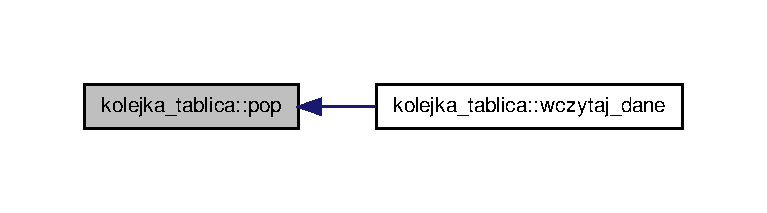
\includegraphics[width=350pt]{classkolejka__tablica_acba0b7dffe0511cf500dc7b4e1bcb3ee_icgraph}
\end{center}
\end{figure}


\hypertarget{classkolejka__tablica_a080e798ff0e2f7168b41c96f3e46753a}{\index{kolejka\-\_\-tablica@{kolejka\-\_\-tablica}!push@{push}}
\index{push@{push}!kolejka_tablica@{kolejka\-\_\-tablica}}
\subsubsection[{push}]{\setlength{\rightskip}{0pt plus 5cm}void kolejka\-\_\-tablica\-::push (
\begin{DoxyParamCaption}
\item[{int}]{element}
\end{DoxyParamCaption}
)}}\label{classkolejka__tablica_a080e798ff0e2f7168b41c96f3e46753a}


Funkcja dodajaca element. 

Funkcja dodaje do stosu element podany przez uzytkownika Funkcja dodaje element poprzez zwiekszenie rozmiaru tablicy o jeden. 
\begin{DoxyParams}{Parameters}
{\em element} & -\/ pole typu int przechowuje wartosc jaka ma byc wpisana \\
\hline
\end{DoxyParams}


Definition at line 17 of file kolejka\-\_\-tablica.\-cpp.



Here is the caller graph for this function\-:\nopagebreak
\begin{figure}[H]
\begin{center}
\leavevmode
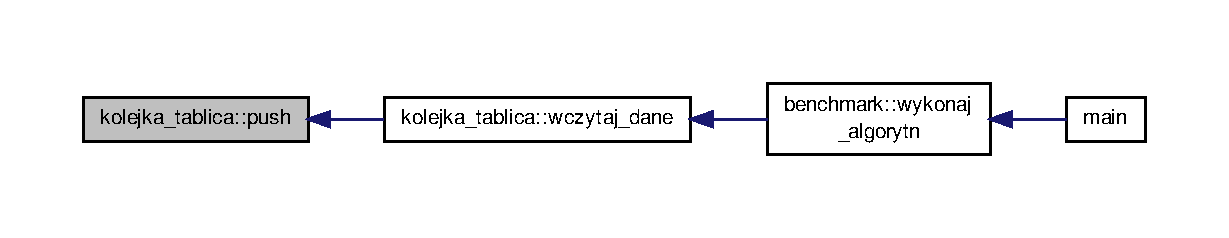
\includegraphics[width=350pt]{classkolejka__tablica_a080e798ff0e2f7168b41c96f3e46753a_icgraph}
\end{center}
\end{figure}


\hypertarget{classkolejka__tablica_ae08cb58ee66340aeb5ef7462eaf05ed8}{\index{kolejka\-\_\-tablica@{kolejka\-\_\-tablica}!pushx2@{pushx2}}
\index{pushx2@{pushx2}!kolejka_tablica@{kolejka\-\_\-tablica}}
\subsubsection[{pushx2}]{\setlength{\rightskip}{0pt plus 5cm}void kolejka\-\_\-tablica\-::pushx2 (
\begin{DoxyParamCaption}
\item[{int}]{element}
\end{DoxyParamCaption}
)}}\label{classkolejka__tablica_ae08cb58ee66340aeb5ef7462eaf05ed8}


Funkcja dodajaca element. 

Funkcja dodaje do stosu element podany przez uzytkownika Funkcja dodaje element poprzez zwiekszenie rozmiaru tablicy o dwa razy niz aktualny stan. 
\begin{DoxyParams}{Parameters}
{\em element} & -\/ pole typu int przechowuje wartosc jaka ma byc wpisana \\
\hline
\end{DoxyParams}


Definition at line 44 of file kolejka\-\_\-tablica.\-cpp.



Here is the caller graph for this function\-:\nopagebreak
\begin{figure}[H]
\begin{center}
\leavevmode
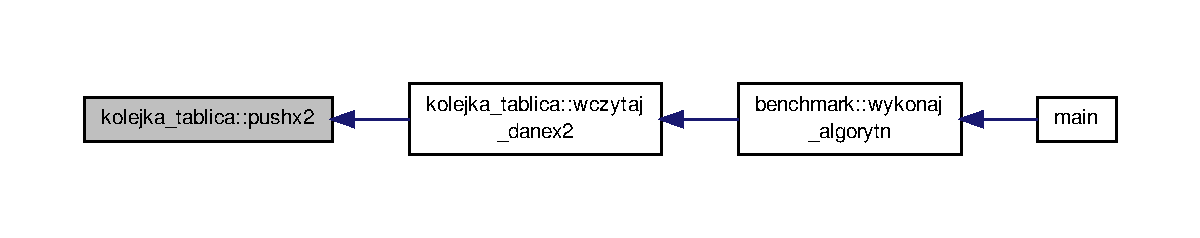
\includegraphics[width=350pt]{classkolejka__tablica_ae08cb58ee66340aeb5ef7462eaf05ed8_icgraph}
\end{center}
\end{figure}


\hypertarget{classkolejka__tablica_a6073b1f832606e6ff706577bc2699338}{\index{kolejka\-\_\-tablica@{kolejka\-\_\-tablica}!size@{size}}
\index{size@{size}!kolejka_tablica@{kolejka\-\_\-tablica}}
\subsubsection[{size}]{\setlength{\rightskip}{0pt plus 5cm}unsigned kolejka\-\_\-tablica\-::size (
\begin{DoxyParamCaption}
{}
\end{DoxyParamCaption}
)}}\label{classkolejka__tablica_a6073b1f832606e6ff706577bc2699338}


Funkcja sprawdzania rozmiar kolejki. 

Funkcja podaje aktualny rozmiar kolejki

\begin{DoxyReturn}{Returns}
rozmiar -\/$>$ rozmiar kolejki 
\end{DoxyReturn}


Definition at line 12 of file kolejka\-\_\-tablica.\-cpp.

\hypertarget{classkolejka__tablica_af0bad5bef2d63767aff69de565026fd2}{\index{kolejka\-\_\-tablica@{kolejka\-\_\-tablica}!wczytaj\-\_\-dane@{wczytaj\-\_\-dane}}
\index{wczytaj\-\_\-dane@{wczytaj\-\_\-dane}!kolejka_tablica@{kolejka\-\_\-tablica}}
\subsubsection[{wczytaj\-\_\-dane}]{\setlength{\rightskip}{0pt plus 5cm}void kolejka\-\_\-tablica\-::wczytaj\-\_\-dane (
\begin{DoxyParamCaption}
{}
\end{DoxyParamCaption}
)}}\label{classkolejka__tablica_af0bad5bef2d63767aff69de565026fd2}


Funkcja wczytywania. 

Funkcja wczytuje wartosci do tabeli z podanego pliku przez uzytkownika. 

Definition at line 107 of file kolejka\-\_\-tablica.\-cpp.



Here is the call graph for this function\-:\nopagebreak
\begin{figure}[H]
\begin{center}
\leavevmode
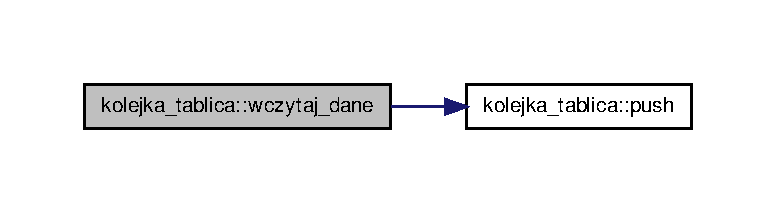
\includegraphics[width=350pt]{classkolejka__tablica_af0bad5bef2d63767aff69de565026fd2_cgraph}
\end{center}
\end{figure}




Here is the caller graph for this function\-:\nopagebreak
\begin{figure}[H]
\begin{center}
\leavevmode
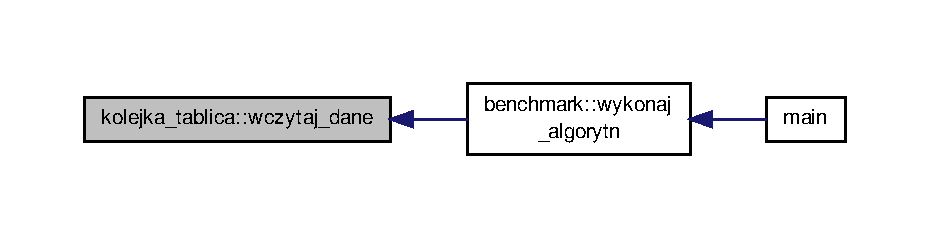
\includegraphics[width=350pt]{classkolejka__tablica_af0bad5bef2d63767aff69de565026fd2_icgraph}
\end{center}
\end{figure}


\hypertarget{classkolejka__tablica_a228697894cc79cea2e5555d624989b1d}{\index{kolejka\-\_\-tablica@{kolejka\-\_\-tablica}!wczytaj\-\_\-dane@{wczytaj\-\_\-dane}}
\index{wczytaj\-\_\-dane@{wczytaj\-\_\-dane}!kolejka_tablica@{kolejka\-\_\-tablica}}
\subsubsection[{wczytaj\-\_\-dane}]{\setlength{\rightskip}{0pt plus 5cm}void kolejka\-\_\-tablica\-::wczytaj\-\_\-dane (
\begin{DoxyParamCaption}
\item[{string}]{nazwa}
\end{DoxyParamCaption}
)}}\label{classkolejka__tablica_a228697894cc79cea2e5555d624989b1d}


Funkcja wczytywania. 

Funkcja wczytuje wartosci do tabeli po przez wpisanie nazwy jako argument metody Wykorzystuje metode push jako funkcje wpisujaca do kolejki


\begin{DoxyParams}{Parameters}
{\em nazwa} & -\/$>$ zmienna typu string, przechowuje nazwe otwieranego pliku \\
\hline
\end{DoxyParams}


Definition at line 124 of file kolejka\-\_\-tablica.\-cpp.



Here is the call graph for this function\-:\nopagebreak
\begin{figure}[H]
\begin{center}
\leavevmode
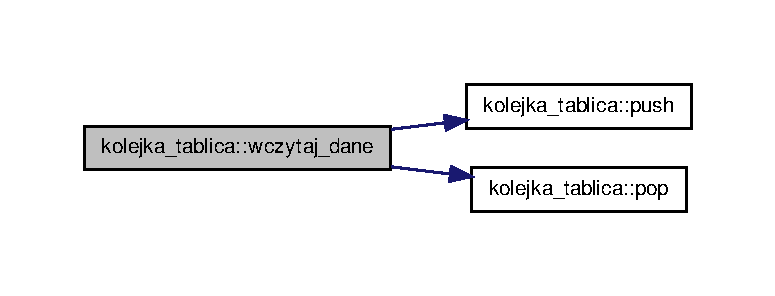
\includegraphics[width=350pt]{classkolejka__tablica_a228697894cc79cea2e5555d624989b1d_cgraph}
\end{center}
\end{figure}


\hypertarget{classkolejka__tablica_a997d0fa8aa2ff8eb838998a82353d828}{\index{kolejka\-\_\-tablica@{kolejka\-\_\-tablica}!wczytaj\-\_\-danex2@{wczytaj\-\_\-danex2}}
\index{wczytaj\-\_\-danex2@{wczytaj\-\_\-danex2}!kolejka_tablica@{kolejka\-\_\-tablica}}
\subsubsection[{wczytaj\-\_\-danex2}]{\setlength{\rightskip}{0pt plus 5cm}void kolejka\-\_\-tablica\-::wczytaj\-\_\-danex2 (
\begin{DoxyParamCaption}
\item[{string}]{nazwa}
\end{DoxyParamCaption}
)}}\label{classkolejka__tablica_a997d0fa8aa2ff8eb838998a82353d828}


Funkcja wczytywania. 

Funkcja wczytuje wartosci do tabeli po przez wpisanie nazwy jako argument metody Wykorzystuje metode pushx2 jako funkcje wpisujaca do kolejki


\begin{DoxyParams}{Parameters}
{\em nazwa} & -\/$>$ zmienna typu string, przechowuje nazwe otwieranego pliku \\
\hline
\end{DoxyParams}


Definition at line 140 of file kolejka\-\_\-tablica.\-cpp.



Here is the call graph for this function\-:\nopagebreak
\begin{figure}[H]
\begin{center}
\leavevmode
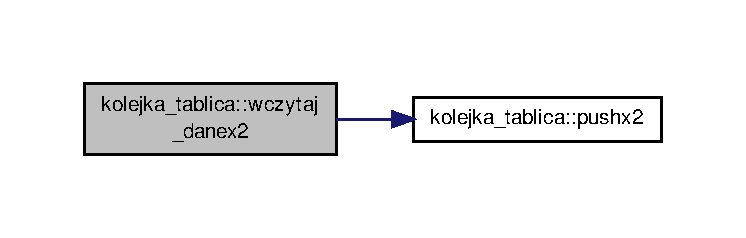
\includegraphics[width=350pt]{classkolejka__tablica_a997d0fa8aa2ff8eb838998a82353d828_cgraph}
\end{center}
\end{figure}




Here is the caller graph for this function\-:\nopagebreak
\begin{figure}[H]
\begin{center}
\leavevmode
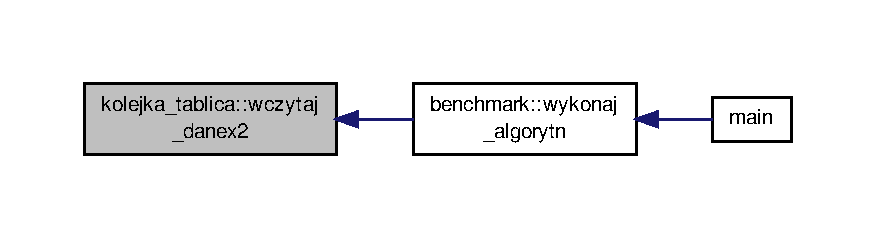
\includegraphics[width=350pt]{classkolejka__tablica_a997d0fa8aa2ff8eb838998a82353d828_icgraph}
\end{center}
\end{figure}




\subsection{Member Data Documentation}
\hypertarget{classkolejka__tablica_a3db25a7939b4a9d96127b29b753d9010}{\index{kolejka\-\_\-tablica@{kolejka\-\_\-tablica}!dane@{dane}}
\index{dane@{dane}!kolejka_tablica@{kolejka\-\_\-tablica}}
\subsubsection[{dane}]{\setlength{\rightskip}{0pt plus 5cm}int$\ast$ kolejka\-\_\-tablica\-::dane\hspace{0.3cm}{\ttfamily [private]}}}\label{classkolejka__tablica_a3db25a7939b4a9d96127b29b753d9010}


Pole typu int, bedzie uzywane jako kolejki z danymi. 



Definition at line 35 of file kolejka\-\_\-tablica.\-hh.

\hypertarget{classkolejka__tablica_a3701ca21511ad3acdecf4cce08625eba}{\index{kolejka\-\_\-tablica@{kolejka\-\_\-tablica}!danetmp@{danetmp}}
\index{danetmp@{danetmp}!kolejka_tablica@{kolejka\-\_\-tablica}}
\subsubsection[{danetmp}]{\setlength{\rightskip}{0pt plus 5cm}int$\ast$ kolejka\-\_\-tablica\-::danetmp\hspace{0.3cm}{\ttfamily [private]}}}\label{classkolejka__tablica_a3701ca21511ad3acdecf4cce08625eba}


Pole typu int, bedzie uzywane jako kolejko z danymi sprawdzajacymi, pomocniczymi. 



Definition at line 39 of file kolejka\-\_\-tablica.\-hh.

\hypertarget{classkolejka__tablica_a1cec0ee294c7afb2c6b7ba5589cb8e38}{\index{kolejka\-\_\-tablica@{kolejka\-\_\-tablica}!rozmiar@{rozmiar}}
\index{rozmiar@{rozmiar}!kolejka_tablica@{kolejka\-\_\-tablica}}
\subsubsection[{rozmiar}]{\setlength{\rightskip}{0pt plus 5cm}int kolejka\-\_\-tablica\-::rozmiar\hspace{0.3cm}{\ttfamily [private]}}}\label{classkolejka__tablica_a1cec0ee294c7afb2c6b7ba5589cb8e38}


Pole typu int, bedzie uzywane jako rozmiar tabeli. 



Definition at line 44 of file kolejka\-\_\-tablica.\-hh.

\hypertarget{classkolejka__tablica_afbf8e02fb0cbdc2674fc68da04d8202d}{\index{kolejka\-\_\-tablica@{kolejka\-\_\-tablica}!spr@{spr}}
\index{spr@{spr}!kolejka_tablica@{kolejka\-\_\-tablica}}
\subsubsection[{spr}]{\setlength{\rightskip}{0pt plus 5cm}int kolejka\-\_\-tablica\-::spr\hspace{0.3cm}{\ttfamily [private]}}}\label{classkolejka__tablica_afbf8e02fb0cbdc2674fc68da04d8202d}


Pole typu int, bedzie uzywane jako pomocnicza wartosc jako rozmiar kolejki. 



Definition at line 48 of file kolejka\-\_\-tablica.\-hh.



The documentation for this class was generated from the following files\-:\begin{DoxyCompactItemize}
\item 
/home/pawel/\-Dokumenty/programowanie/pamsi/zad3/prj/inc/\hyperlink{kolejka__tablica_8hh}{kolejka\-\_\-tablica.\-hh}\item 
/home/pawel/\-Dokumenty/programowanie/pamsi/zad3/prj/src/\hyperlink{kolejka__tablica_8cpp}{kolejka\-\_\-tablica.\-cpp}\end{DoxyCompactItemize}

\hypertarget{classstos__lista}{\section{stos\-\_\-lista Class Reference}
\label{classstos__lista}\index{stos\-\_\-lista@{stos\-\_\-lista}}
}


Modeluje pojecie Stos.  




{\ttfamily \#include $<$stos\-\_\-lista.\-hh$>$}



Collaboration diagram for stos\-\_\-lista\-:\nopagebreak
\begin{figure}[H]
\begin{center}
\leavevmode
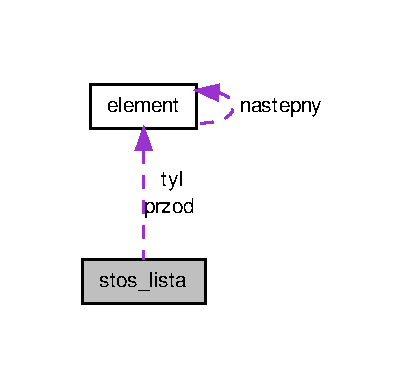
\includegraphics[width=195pt]{classstos__lista__coll__graph}
\end{center}
\end{figure}
\subsection*{Public Member Functions}
\begin{DoxyCompactItemize}
\item 
\hyperlink{classstos__lista_af779e46538f7fec8b2ecdd6469ead07c}{stos\-\_\-lista} ()
\begin{DoxyCompactList}\small\item\em Konstruktor klasy stos. \end{DoxyCompactList}\item 
\hyperlink{classstos__lista_a41eabf2ed23d39a334345484896857ed}{$\sim$stos\-\_\-lista} ()
\begin{DoxyCompactList}\small\item\em Destruktor klasy stos. \end{DoxyCompactList}\item 
void \hyperlink{classstos__lista_a33781da85b24ffc9d6a6f5b470eaa654}{wczytaj\-\_\-dane} ()
\begin{DoxyCompactList}\small\item\em Funkcja wczytywania. \end{DoxyCompactList}\item 
void \hyperlink{classstos__lista_a3ee1e31107ca47737451d808c85f2167}{wczytaj\-\_\-dane} (string nazwa)
\begin{DoxyCompactList}\small\item\em Funkcja wczytywania. \end{DoxyCompactList}\item 
void \hyperlink{classstos__lista_afd27e50bafd3f39fec49568522cc61b2}{pokaz\-\_\-elementy} ()
\begin{DoxyCompactList}\small\item\em Funkcja wyswietlajaca. \end{DoxyCompactList}\item 
bool \hyperlink{classstos__lista_abce2b3948d8a5dd5f62bfc985d97fe54}{isempty} ()
\begin{DoxyCompactList}\small\item\em Funkcja sprawdzania pustosci stosu. \end{DoxyCompactList}\item 
unsigned \hyperlink{classstos__lista_a36fa9223746729efa49ffad6001e87ae}{size} ()
\begin{DoxyCompactList}\small\item\em Funkcja sprawdzania rozmiar stosu. \end{DoxyCompactList}\item 
\hyperlink{classelement}{element} $\ast$ \hyperlink{classstos__lista_ad38186a811405f247940c262073744f1}{push} (\hyperlink{classelement}{element} $\ast$p)
\begin{DoxyCompactList}\small\item\em Funkcja dodajaca element. \end{DoxyCompactList}\item 
void \hyperlink{classstos__lista_af461edd89f331e301d02460dc330b4e5}{dodaj\-\_\-element} (int a)
\begin{DoxyCompactList}\small\item\em Funkcja dodajaca element. \end{DoxyCompactList}\item 
\hyperlink{classelement}{element} $\ast$ \hyperlink{classstos__lista_af637e1d174c0f0005e0157b6dc35c41a}{pop} ()
\begin{DoxyCompactList}\small\item\em Funkcja usuwajaca ostatni element ze stosu. \end{DoxyCompactList}\end{DoxyCompactItemize}
\subsection*{Private Attributes}
\begin{DoxyCompactItemize}
\item 
\hyperlink{classelement}{element} $\ast$ \hyperlink{classstos__lista_ad9cd66242f8b8342bb3d8cb5852f58c5}{przod}
\begin{DoxyCompactList}\small\item\em Pole typu element, wskazuje na pierwszy element listy. \end{DoxyCompactList}\item 
\hyperlink{classelement}{element} $\ast$ \hyperlink{classstos__lista_af724a08b1601250dfc1a333430be9515}{tyl}
\begin{DoxyCompactList}\small\item\em Pole typu element, wskazuje na ostatni element listy. \end{DoxyCompactList}\item 
unsigned \hyperlink{classstos__lista_ab9d47f55d1288d44e0b58fcea281925f}{licznik}
\begin{DoxyCompactList}\small\item\em Pole typu int, bedzie uzywane jako rozmiar stosu. \end{DoxyCompactList}\end{DoxyCompactItemize}


\subsection{Detailed Description}
Modeluje pojecie Stos. 

Stos jest klasa zawierajaca dynamicznie zaalokowane lista 

Definition at line 53 of file stos\-\_\-lista.\-hh.



\subsection{Constructor \& Destructor Documentation}
\hypertarget{classstos__lista_af779e46538f7fec8b2ecdd6469ead07c}{\index{stos\-\_\-lista@{stos\-\_\-lista}!stos\-\_\-lista@{stos\-\_\-lista}}
\index{stos\-\_\-lista@{stos\-\_\-lista}!stos_lista@{stos\-\_\-lista}}
\subsubsection[{stos\-\_\-lista}]{\setlength{\rightskip}{0pt plus 5cm}stos\-\_\-lista\-::stos\-\_\-lista (
\begin{DoxyParamCaption}
{}
\end{DoxyParamCaption}
)\hspace{0.3cm}{\ttfamily [inline]}}}\label{classstos__lista_af779e46538f7fec8b2ecdd6469ead07c}


Konstruktor klasy stos. 

Konstruktor jest bezparametryczny, inicjalizuje wszystkie skladowe klasy wartosciami zerowymi. 

Definition at line 79 of file stos\-\_\-lista.\-hh.

\hypertarget{classstos__lista_a41eabf2ed23d39a334345484896857ed}{\index{stos\-\_\-lista@{stos\-\_\-lista}!$\sim$stos\-\_\-lista@{$\sim$stos\-\_\-lista}}
\index{$\sim$stos\-\_\-lista@{$\sim$stos\-\_\-lista}!stos_lista@{stos\-\_\-lista}}
\subsubsection[{$\sim$stos\-\_\-lista}]{\setlength{\rightskip}{0pt plus 5cm}stos\-\_\-lista\-::$\sim$stos\-\_\-lista (
\begin{DoxyParamCaption}
{}
\end{DoxyParamCaption}
)\hspace{0.3cm}{\ttfamily [inline]}}}\label{classstos__lista_a41eabf2ed23d39a334345484896857ed}


Destruktor klasy stos. 

Usuwa dynamicznie zaalokawana liste 

Definition at line 86 of file stos\-\_\-lista.\-hh.



\subsection{Member Function Documentation}
\hypertarget{classstos__lista_af461edd89f331e301d02460dc330b4e5}{\index{stos\-\_\-lista@{stos\-\_\-lista}!dodaj\-\_\-element@{dodaj\-\_\-element}}
\index{dodaj\-\_\-element@{dodaj\-\_\-element}!stos_lista@{stos\-\_\-lista}}
\subsubsection[{dodaj\-\_\-element}]{\setlength{\rightskip}{0pt plus 5cm}void stos\-\_\-lista\-::dodaj\-\_\-element (
\begin{DoxyParamCaption}
\item[{int}]{a}
\end{DoxyParamCaption}
)}}\label{classstos__lista_af461edd89f331e301d02460dc330b4e5}


Funkcja dodajaca element. 

Funkcja dodaje do stosu element podany przez uzytkownika poprzez wywolanie funkcji \hyperlink{classstos__lista_ad38186a811405f247940c262073744f1}{push()}. 
\begin{DoxyParams}{Parameters}
{\em a} & -\/ pole typu int przechowuje wartosc jaka ma byc wpisana \\
\hline
\end{DoxyParams}


Definition at line 61 of file stos\-\_\-lista.\-cpp.

\hypertarget{classstos__lista_abce2b3948d8a5dd5f62bfc985d97fe54}{\index{stos\-\_\-lista@{stos\-\_\-lista}!isempty@{isempty}}
\index{isempty@{isempty}!stos_lista@{stos\-\_\-lista}}
\subsubsection[{isempty}]{\setlength{\rightskip}{0pt plus 5cm}bool stos\-\_\-lista\-::isempty (
\begin{DoxyParamCaption}
{}
\end{DoxyParamCaption}
)}}\label{classstos__lista_abce2b3948d8a5dd5f62bfc985d97fe54}


Funkcja sprawdzania pustosci stosu. 

Funkcja sprawdza czy stos jest pusty

\begin{DoxyReturn}{Returns}
1 -\/$>$ Stos pusty \par
 0 -\/$>$ Stos nie pusty 
\end{DoxyReturn}


Definition at line 7 of file stos\-\_\-lista.\-cpp.

\hypertarget{classstos__lista_afd27e50bafd3f39fec49568522cc61b2}{\index{stos\-\_\-lista@{stos\-\_\-lista}!pokaz\-\_\-elementy@{pokaz\-\_\-elementy}}
\index{pokaz\-\_\-elementy@{pokaz\-\_\-elementy}!stos_lista@{stos\-\_\-lista}}
\subsubsection[{pokaz\-\_\-elementy}]{\setlength{\rightskip}{0pt plus 5cm}void stos\-\_\-lista\-::pokaz\-\_\-elementy (
\begin{DoxyParamCaption}
{}
\end{DoxyParamCaption}
)}}\label{classstos__lista_afd27e50bafd3f39fec49568522cc61b2}


Funkcja wyswietlajaca. 

Funkcja wyswietla aktualny stan stosu 

Definition at line 44 of file stos\-\_\-lista.\-cpp.

\hypertarget{classstos__lista_af637e1d174c0f0005e0157b6dc35c41a}{\index{stos\-\_\-lista@{stos\-\_\-lista}!pop@{pop}}
\index{pop@{pop}!stos_lista@{stos\-\_\-lista}}
\subsubsection[{pop}]{\setlength{\rightskip}{0pt plus 5cm}{\bf element} $\ast$ stos\-\_\-lista\-::pop (
\begin{DoxyParamCaption}
{}
\end{DoxyParamCaption}
)}}\label{classstos__lista_af637e1d174c0f0005e0157b6dc35c41a}


Funkcja usuwajaca ostatni element ze stosu. 

Funkcja usuwa z listy pierwszy element i zwraca jego adres. Element zostaje jedynie odłączony od listy, lecz wciąż zajmuje swój obszar pamięci.

Na początku sprawdzamy, czy lista zawiera jakiś element. Jeśli nie, zwracamy N\-U\-L\-L. W przeciwnym razie zapamiętujemy w zmiennej p adres pierwszego elementu. W polu przod umieszczamy adres następnego elementu listy. W ten sposób element p zostaje odłączony logicznie od listy.

Jeśli po odłączeniu pole przod zawiera adres N\-U\-L\-L, to lista jest obecnie pusta i N\-U\-L\-L wpisujemy również do pola tyl.

Zmniejszamy o jeden licznik licznik i zwracamy adres usuniętego z listy elementu. 

Definition at line 28 of file stos\-\_\-lista.\-cpp.

\hypertarget{classstos__lista_ad38186a811405f247940c262073744f1}{\index{stos\-\_\-lista@{stos\-\_\-lista}!push@{push}}
\index{push@{push}!stos_lista@{stos\-\_\-lista}}
\subsubsection[{push}]{\setlength{\rightskip}{0pt plus 5cm}{\bf element} $\ast$ stos\-\_\-lista\-::push (
\begin{DoxyParamCaption}
\item[{{\bf element} $\ast$}]{p}
\end{DoxyParamCaption}
)}}\label{classstos__lista_ad38186a811405f247940c262073744f1}


Funkcja dodajaca element. 

Funkcja wstawia nowy element p na początek listy i zwraca jego adres.

Najpierw wpisuje w pole nastpeny elementu p adres pierwszego elementu listy. W efekcie pierwszy element listy staje się elementem następnym dla p. W polu przod zostaje umieszczony adres elementu p, czyli staje się on pierwszym elementem na liście.

Lista mogła być pusta. Jeśli pole tyl zawiera N\-U\-L\-L, to wstawiony element jest jedynym jak dotąd elementem listy. Zatem jest on zarówno elementem pierwszym jak i ostatnim. Dlatego w polu tyl umieszczamy w tym przypadku adres pierwszego elementu pobrany z pola przod.

Po wstawieniu elementu zwiększamy licznik licznik i zwracamy adres pierwszego elementu listy.


\begin{DoxyParams}{Parameters}
{\em p} & -\/ pole typu element przechowuje wartosc jaka ma byc wpisana \\
\hline
\end{DoxyParams}
\begin{DoxyReturn}{Returns}
adres nowego elementu. 
\end{DoxyReturn}


Definition at line 20 of file stos\-\_\-lista.\-cpp.

\hypertarget{classstos__lista_a36fa9223746729efa49ffad6001e87ae}{\index{stos\-\_\-lista@{stos\-\_\-lista}!size@{size}}
\index{size@{size}!stos_lista@{stos\-\_\-lista}}
\subsubsection[{size}]{\setlength{\rightskip}{0pt plus 5cm}unsigned stos\-\_\-lista\-::size (
\begin{DoxyParamCaption}
{}
\end{DoxyParamCaption}
)}}\label{classstos__lista_a36fa9223746729efa49ffad6001e87ae}


Funkcja sprawdzania rozmiar stosu. 

Funkcja podaje aktualny rozmiar stosu

\begin{DoxyReturn}{Returns}
rozmiar -\/$>$ rozmiar stosu 
\end{DoxyReturn}


Definition at line 15 of file stos\-\_\-lista.\-cpp.

\hypertarget{classstos__lista_a33781da85b24ffc9d6a6f5b470eaa654}{\index{stos\-\_\-lista@{stos\-\_\-lista}!wczytaj\-\_\-dane@{wczytaj\-\_\-dane}}
\index{wczytaj\-\_\-dane@{wczytaj\-\_\-dane}!stos_lista@{stos\-\_\-lista}}
\subsubsection[{wczytaj\-\_\-dane}]{\setlength{\rightskip}{0pt plus 5cm}void stos\-\_\-lista\-::wczytaj\-\_\-dane (
\begin{DoxyParamCaption}
{}
\end{DoxyParamCaption}
)}}\label{classstos__lista_a33781da85b24ffc9d6a6f5b470eaa654}


Funkcja wczytywania. 

Funkcja wczytuje wartosci do stosu z podanego pliku przez uzytkownika. 

Definition at line 68 of file stos\-\_\-lista.\-cpp.



Here is the caller graph for this function\-:\nopagebreak
\begin{figure}[H]
\begin{center}
\leavevmode
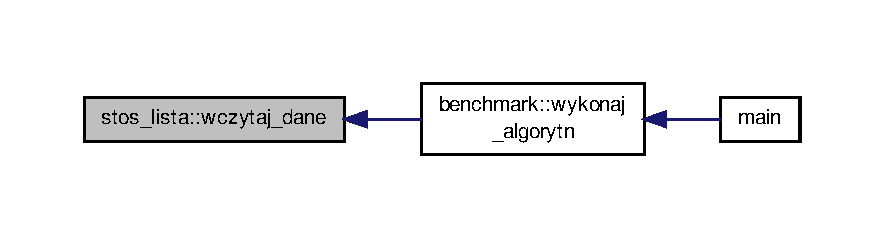
\includegraphics[width=350pt]{classstos__lista_a33781da85b24ffc9d6a6f5b470eaa654_icgraph}
\end{center}
\end{figure}


\hypertarget{classstos__lista_a3ee1e31107ca47737451d808c85f2167}{\index{stos\-\_\-lista@{stos\-\_\-lista}!wczytaj\-\_\-dane@{wczytaj\-\_\-dane}}
\index{wczytaj\-\_\-dane@{wczytaj\-\_\-dane}!stos_lista@{stos\-\_\-lista}}
\subsubsection[{wczytaj\-\_\-dane}]{\setlength{\rightskip}{0pt plus 5cm}void stos\-\_\-lista\-::wczytaj\-\_\-dane (
\begin{DoxyParamCaption}
\item[{string}]{nazwa}
\end{DoxyParamCaption}
)}}\label{classstos__lista_a3ee1e31107ca47737451d808c85f2167}


Funkcja wczytywania. 

Funkcja wczytuje wartosci do tabeli po przez wpisanie nazwy jako argument metody Wykorzystuje metode push jako funkcje wpisujaca do stosu


\begin{DoxyParams}{Parameters}
{\em nazwa} & -\/$>$ zmienna typu string, przechowuje nazwe otwieranego pliku \\
\hline
\end{DoxyParams}


Definition at line 85 of file stos\-\_\-lista.\-cpp.



\subsection{Member Data Documentation}
\hypertarget{classstos__lista_ab9d47f55d1288d44e0b58fcea281925f}{\index{stos\-\_\-lista@{stos\-\_\-lista}!licznik@{licznik}}
\index{licznik@{licznik}!stos_lista@{stos\-\_\-lista}}
\subsubsection[{licznik}]{\setlength{\rightskip}{0pt plus 5cm}unsigned stos\-\_\-lista\-::licznik\hspace{0.3cm}{\ttfamily [private]}}}\label{classstos__lista_ab9d47f55d1288d44e0b58fcea281925f}


Pole typu int, bedzie uzywane jako rozmiar stosu. 



Definition at line 68 of file stos\-\_\-lista.\-hh.

\hypertarget{classstos__lista_ad9cd66242f8b8342bb3d8cb5852f58c5}{\index{stos\-\_\-lista@{stos\-\_\-lista}!przod@{przod}}
\index{przod@{przod}!stos_lista@{stos\-\_\-lista}}
\subsubsection[{przod}]{\setlength{\rightskip}{0pt plus 5cm}{\bf element}$\ast$ stos\-\_\-lista\-::przod\hspace{0.3cm}{\ttfamily [private]}}}\label{classstos__lista_ad9cd66242f8b8342bb3d8cb5852f58c5}


Pole typu element, wskazuje na pierwszy element listy. 



Definition at line 59 of file stos\-\_\-lista.\-hh.

\hypertarget{classstos__lista_af724a08b1601250dfc1a333430be9515}{\index{stos\-\_\-lista@{stos\-\_\-lista}!tyl@{tyl}}
\index{tyl@{tyl}!stos_lista@{stos\-\_\-lista}}
\subsubsection[{tyl}]{\setlength{\rightskip}{0pt plus 5cm}{\bf element}$\ast$ stos\-\_\-lista\-::tyl\hspace{0.3cm}{\ttfamily [private]}}}\label{classstos__lista_af724a08b1601250dfc1a333430be9515}


Pole typu element, wskazuje na ostatni element listy. 



Definition at line 63 of file stos\-\_\-lista.\-hh.



The documentation for this class was generated from the following files\-:\begin{DoxyCompactItemize}
\item 
/home/pawel/\-Dokumenty/programowanie/pamsi/zad3/prj/inc/\hyperlink{stos__lista_8hh}{stos\-\_\-lista.\-hh}\item 
/home/pawel/\-Dokumenty/programowanie/pamsi/zad3/prj/src/\hyperlink{stos__lista_8cpp}{stos\-\_\-lista.\-cpp}\end{DoxyCompactItemize}

\hypertarget{classstos__tablica}{\section{stos\-\_\-tablica Class Reference}
\label{classstos__tablica}\index{stos\-\_\-tablica@{stos\-\_\-tablica}}
}


Modeluje pojecie Stos.  




{\ttfamily \#include $<$stos\-\_\-tablica.\-hh$>$}

\subsection*{Public Member Functions}
\begin{DoxyCompactItemize}
\item 
\hyperlink{classstos__tablica_a7dfdcb1a98f9434a5f94ebc19ac14af5}{stos\-\_\-tablica} ()
\begin{DoxyCompactList}\small\item\em Konstruktor klasy stos. \end{DoxyCompactList}\item 
\hyperlink{classstos__tablica_a684a8f468cb76ecf6c01df66fcbae8f6}{$\sim$stos\-\_\-tablica} ()
\begin{DoxyCompactList}\small\item\em Destruktor klasy stos. \end{DoxyCompactList}\item 
void \hyperlink{classstos__tablica_a68d7d3ed8622663ff7aca3b9696724c5}{wczytaj\-\_\-dane} ()
\begin{DoxyCompactList}\small\item\em Funkcja wczytywania. \end{DoxyCompactList}\item 
void \hyperlink{classstos__tablica_a33b9257de4213c84e96e666898f5ead0}{wczytaj\-\_\-dane} (string nazwa)
\begin{DoxyCompactList}\small\item\em Funkcja wczytywania. \end{DoxyCompactList}\item 
void \hyperlink{classstos__tablica_a89f6cd04da8bafdded7b8d0f003e3978}{pokaz\-\_\-elementy} ()
\begin{DoxyCompactList}\small\item\em Funkcja wyswietlajaca. \end{DoxyCompactList}\item 
int \hyperlink{classstos__tablica_a29bd76c04019f6b149090a8882d54f7b}{get\-\_\-rozmiar} ()
\begin{DoxyCompactList}\small\item\em Funkcja sprawdzania rozmiar stosu. \end{DoxyCompactList}\item 
void \hyperlink{classstos__tablica_a340038b0ac6af3983de3fe21fa54aa36}{quicksort} (int left, int right)
\begin{DoxyCompactList}\small\item\em Funkcja sortujaca. \end{DoxyCompactList}\item 
void \hyperlink{classstos__tablica_a636f59632a29c985a404c0c8a3a9a18f}{quick\-\_\-sort} ()
\begin{DoxyCompactList}\small\item\em Funkcja wywolujaca funkcje sorujaca Quick Sort. \end{DoxyCompactList}\item 
void \hyperlink{classstos__tablica_a64e273a78434133331b24a4f9bbff87b}{swap} (int $\ast$x, int $\ast$y)
\begin{DoxyCompactList}\small\item\em Funkcja zamieniania wartosci. \end{DoxyCompactList}\item 
void \hyperlink{classstos__tablica_abeeb3fc4e2bc9a9b9917b3e996eb388e}{wypelnij\-\_\-losowo} ()
\begin{DoxyCompactList}\small\item\em Funkcja wypelniajaca stos losowymi wartosciami. \end{DoxyCompactList}\item 
void \hyperlink{classstos__tablica_a430a06f13dc5a74bca50b07cc993196c}{wyzeruj\-\_\-stos} ()
\begin{DoxyCompactList}\small\item\em Funkcja zerujaca stos. \end{DoxyCompactList}\item 
void \hyperlink{classstos__tablica_aabebf0add57a2440cddd9b4305d165f8}{wyzeruj\-\_\-stos\-\_\-caly} ()
\begin{DoxyCompactList}\small\item\em Funkcja zerujaca caly stos. \end{DoxyCompactList}\item 
int \hyperlink{classstos__tablica_a688f873f65a862620d11b92f9d52c685}{get\-\_\-lewy} ()
\begin{DoxyCompactList}\small\item\em Funkcja dostepu do prywantego pola klasy lewy. \end{DoxyCompactList}\item 
int \hyperlink{classstos__tablica_aa8c6fdb7c9214f9235dbc896a9c53581}{get\-\_\-prawy} ()
\begin{DoxyCompactList}\small\item\em Funkcja dostepu do prywantego pola klasy prawy. \end{DoxyCompactList}\item 
void \hyperlink{classstos__tablica_a79d983833ba1481654c51787bb604936}{mergesort} (int pocz, int kon)
\begin{DoxyCompactList}\small\item\em Funkcja sortujaca. \end{DoxyCompactList}\item 
void \hyperlink{classstos__tablica_afaad303fc8eef3b5c115d5da31c38bc1}{merge\-\_\-sort} ()
\begin{DoxyCompactList}\small\item\em Funkcja wywolujaca funkcje sorujaca Merge Sort. \end{DoxyCompactList}\item 
void \hyperlink{classstos__tablica_a3e932a92382d6befc649da95561b99ce}{build\-\_\-heap} ()
\begin{DoxyCompactList}\small\item\em Funkcja budujaca kopiec ( Heap ). \end{DoxyCompactList}\item 
void \hyperlink{classstos__tablica_aa3a60813771d70e2d9c8f2cab195964c}{disassemble\-\_\-heap} ()
\begin{DoxyCompactList}\small\item\em Funkcja rozbierajaca kopiec ( Heap ). \end{DoxyCompactList}\item 
void \hyperlink{classstos__tablica_a6168dfa3d54b01c4702313329112fb1d}{heap\-\_\-sort} ()
\begin{DoxyCompactList}\small\item\em Funkcja wywolujaca funkcje sorujaca Heap Sort. \end{DoxyCompactList}\item 
void \hyperlink{classstos__tablica_aac88873e08b12ea26661690feb28ea86}{przypisz} ()
\begin{DoxyCompactList}\small\item\em Funkcja przypisujaca. \end{DoxyCompactList}\end{DoxyCompactItemize}
\subsection*{Private Attributes}
\begin{DoxyCompactItemize}
\item 
int $\ast$ \hyperlink{classstos__tablica_a008b0f69384d5d987782c2f24fcbd387}{dane}
\begin{DoxyCompactList}\small\item\em Pole typu int, bedzie uzywane jako stosu z danymi. \end{DoxyCompactList}\item 
int $\ast$ \hyperlink{classstos__tablica_a2ee83414df31c2f56383199a5d47c755}{danetmp}
\begin{DoxyCompactList}\small\item\em Pole typu int, bedzie uzywane jako stosu z danymi sprawdzajacymi, pomocniczymi. \end{DoxyCompactList}\item 
int \hyperlink{classstos__tablica_aa9c1d33bd477174602d2632c74ebea9c}{rozmiar}
\begin{DoxyCompactList}\small\item\em Pole typu int, bedzie uzywane jako rozmiar tabeli. \end{DoxyCompactList}\item 
int \hyperlink{classstos__tablica_adcfe2091d485a93da47eb9fb6a337b06}{rozmiar\-\_\-tmp}
\begin{DoxyCompactList}\small\item\em Pole typu int, bedzie uzywane jako pomocnicza wartosc jako rozmiar stosu. \end{DoxyCompactList}\item 
int \hyperlink{classstos__tablica_addee4392050e497f2b9f07a5e7a17606}{lewy}
\begin{DoxyCompactList}\small\item\em Pole typu int, bedzie uzywane jako pomocnicza wartosc do metody Quick Sort. \end{DoxyCompactList}\item 
int \hyperlink{classstos__tablica_aab32beac5ab0f185fb27492736798749}{prawy}
\begin{DoxyCompactList}\small\item\em Pole typu int, bedzie uzywane jako pomocnicza wartosc do metody Quick Sort. \end{DoxyCompactList}\item 
int \hyperlink{classstos__tablica_ae1737beb175c9041e44ff8b374fa3565}{heap\-\_\-size}
\begin{DoxyCompactList}\small\item\em Pole typu int, bedzie uzywane jako pomocnicza wartosc do metody Heap Size. \end{DoxyCompactList}\end{DoxyCompactItemize}


\subsection{Detailed Description}
Modeluje pojecie Stos. 

Stos jest klasa zawierajaca dynamicznie zaalokowane 2 tablice Pierwsza z nich to tablica z danymi, na ktorych beda wykonywane operacje. Druga z nich sluzy jako tablica do przechowywania tymczasowych danych. 

Definition at line 33 of file stos\-\_\-tablica.\-hh.



\subsection{Constructor \& Destructor Documentation}
\hypertarget{classstos__tablica_a7dfdcb1a98f9434a5f94ebc19ac14af5}{\index{stos\-\_\-tablica@{stos\-\_\-tablica}!stos\-\_\-tablica@{stos\-\_\-tablica}}
\index{stos\-\_\-tablica@{stos\-\_\-tablica}!stos_tablica@{stos\-\_\-tablica}}
\subsubsection[{stos\-\_\-tablica}]{\setlength{\rightskip}{0pt plus 5cm}stos\-\_\-tablica\-::stos\-\_\-tablica (
\begin{DoxyParamCaption}
{}
\end{DoxyParamCaption}
)\hspace{0.3cm}{\ttfamily [inline]}}}\label{classstos__tablica_a7dfdcb1a98f9434a5f94ebc19ac14af5}


Konstruktor klasy stos. 

Konstruktor jest bezparametryczny, inicjalizuje wszystkie skladowe klasy wartosciami zerowymi. 

Definition at line 73 of file stos\-\_\-tablica.\-hh.

\hypertarget{classstos__tablica_a684a8f468cb76ecf6c01df66fcbae8f6}{\index{stos\-\_\-tablica@{stos\-\_\-tablica}!$\sim$stos\-\_\-tablica@{$\sim$stos\-\_\-tablica}}
\index{$\sim$stos\-\_\-tablica@{$\sim$stos\-\_\-tablica}!stos_tablica@{stos\-\_\-tablica}}
\subsubsection[{$\sim$stos\-\_\-tablica}]{\setlength{\rightskip}{0pt plus 5cm}stos\-\_\-tablica\-::$\sim$stos\-\_\-tablica (
\begin{DoxyParamCaption}
{}
\end{DoxyParamCaption}
)\hspace{0.3cm}{\ttfamily [inline]}}}\label{classstos__tablica_a684a8f468cb76ecf6c01df66fcbae8f6}


Destruktor klasy stos. 

Usuwa dynamicznie zaalokawana tablice 

Definition at line 80 of file stos\-\_\-tablica.\-hh.



\subsection{Member Function Documentation}
\hypertarget{classstos__tablica_a3e932a92382d6befc649da95561b99ce}{\index{stos\-\_\-tablica@{stos\-\_\-tablica}!build\-\_\-heap@{build\-\_\-heap}}
\index{build\-\_\-heap@{build\-\_\-heap}!stos_tablica@{stos\-\_\-tablica}}
\subsubsection[{build\-\_\-heap}]{\setlength{\rightskip}{0pt plus 5cm}void stos\-\_\-tablica\-::build\-\_\-heap (
\begin{DoxyParamCaption}
{}
\end{DoxyParamCaption}
)}}\label{classstos__tablica_a3e932a92382d6befc649da95561b99ce}


Funkcja budujaca kopiec ( Heap ). 

Funkcja tworzy kopiec z wstepnie posortowanymi danymi. Reszta zostanie posortowana przy jego rozbieraniu. 

Definition at line 184 of file stos\-\_\-tablica.\-cpp.

\hypertarget{classstos__tablica_aa3a60813771d70e2d9c8f2cab195964c}{\index{stos\-\_\-tablica@{stos\-\_\-tablica}!disassemble\-\_\-heap@{disassemble\-\_\-heap}}
\index{disassemble\-\_\-heap@{disassemble\-\_\-heap}!stos_tablica@{stos\-\_\-tablica}}
\subsubsection[{disassemble\-\_\-heap}]{\setlength{\rightskip}{0pt plus 5cm}void stos\-\_\-tablica\-::disassemble\-\_\-heap (
\begin{DoxyParamCaption}
{}
\end{DoxyParamCaption}
)}}\label{classstos__tablica_aa3a60813771d70e2d9c8f2cab195964c}


Funkcja rozbierajaca kopiec ( Heap ). 

Funkcja rozbiera kopiec, jednoczesnie sortujac dane. 

Definition at line 203 of file stos\-\_\-tablica.\-cpp.

\hypertarget{classstos__tablica_a688f873f65a862620d11b92f9d52c685}{\index{stos\-\_\-tablica@{stos\-\_\-tablica}!get\-\_\-lewy@{get\-\_\-lewy}}
\index{get\-\_\-lewy@{get\-\_\-lewy}!stos_tablica@{stos\-\_\-tablica}}
\subsubsection[{get\-\_\-lewy}]{\setlength{\rightskip}{0pt plus 5cm}int stos\-\_\-tablica\-::get\-\_\-lewy (
\begin{DoxyParamCaption}
{}
\end{DoxyParamCaption}
)\hspace{0.3cm}{\ttfamily [inline]}}}\label{classstos__tablica_a688f873f65a862620d11b92f9d52c685}


Funkcja dostepu do prywantego pola klasy lewy. 

\begin{DoxyReturn}{Returns}
lewy -\/$>$ obiekt typu int, indeks pierwszego elementu stosu ( zazwyczaj 0 ) 
\end{DoxyReturn}


Definition at line 185 of file stos\-\_\-tablica.\-hh.

\hypertarget{classstos__tablica_aa8c6fdb7c9214f9235dbc896a9c53581}{\index{stos\-\_\-tablica@{stos\-\_\-tablica}!get\-\_\-prawy@{get\-\_\-prawy}}
\index{get\-\_\-prawy@{get\-\_\-prawy}!stos_tablica@{stos\-\_\-tablica}}
\subsubsection[{get\-\_\-prawy}]{\setlength{\rightskip}{0pt plus 5cm}int stos\-\_\-tablica\-::get\-\_\-prawy (
\begin{DoxyParamCaption}
{}
\end{DoxyParamCaption}
)\hspace{0.3cm}{\ttfamily [inline]}}}\label{classstos__tablica_aa8c6fdb7c9214f9235dbc896a9c53581}


Funkcja dostepu do prywantego pola klasy prawy. 

\begin{DoxyReturn}{Returns}
prawy -\/$>$ obiekt typu int, indeks ostatniego elementu stosu ( zazwyczaj rowne rozmiarowi ) 
\end{DoxyReturn}


Definition at line 192 of file stos\-\_\-tablica.\-hh.

\hypertarget{classstos__tablica_a29bd76c04019f6b149090a8882d54f7b}{\index{stos\-\_\-tablica@{stos\-\_\-tablica}!get\-\_\-rozmiar@{get\-\_\-rozmiar}}
\index{get\-\_\-rozmiar@{get\-\_\-rozmiar}!stos_tablica@{stos\-\_\-tablica}}
\subsubsection[{get\-\_\-rozmiar}]{\setlength{\rightskip}{0pt plus 5cm}int stos\-\_\-tablica\-::get\-\_\-rozmiar (
\begin{DoxyParamCaption}
{}
\end{DoxyParamCaption}
)\hspace{0.3cm}{\ttfamily [inline]}}}\label{classstos__tablica_a29bd76c04019f6b149090a8882d54f7b}


Funkcja sprawdzania rozmiar stosu. 

Funkcja podaje aktualny rozmiar stosu

\begin{DoxyReturn}{Returns}
rozmiar -\/$>$ rozmiar stosu 
\end{DoxyReturn}


Definition at line 127 of file stos\-\_\-tablica.\-hh.

\hypertarget{classstos__tablica_a6168dfa3d54b01c4702313329112fb1d}{\index{stos\-\_\-tablica@{stos\-\_\-tablica}!heap\-\_\-sort@{heap\-\_\-sort}}
\index{heap\-\_\-sort@{heap\-\_\-sort}!stos_tablica@{stos\-\_\-tablica}}
\subsubsection[{heap\-\_\-sort}]{\setlength{\rightskip}{0pt plus 5cm}void stos\-\_\-tablica\-::heap\-\_\-sort (
\begin{DoxyParamCaption}
{}
\end{DoxyParamCaption}
)\hspace{0.3cm}{\ttfamily [inline]}}}\label{classstos__tablica_a6168dfa3d54b01c4702313329112fb1d}


Funkcja wywolujaca funkcje sorujaca Heap Sort. 

Funkcja jest tylko po to, aby mozna bylo w klasie innej niz ta uruchomic funkcje sortowania jednym poleceniem 

Definition at line 233 of file stos\-\_\-tablica.\-hh.



Here is the caller graph for this function\-:
\nopagebreak
\begin{figure}[H]
\begin{center}
\leavevmode
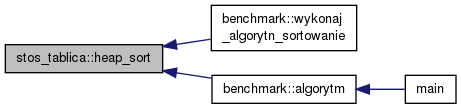
\includegraphics[width=350pt]{classstos__tablica_a6168dfa3d54b01c4702313329112fb1d_icgraph}
\end{center}
\end{figure}


\hypertarget{classstos__tablica_afaad303fc8eef3b5c115d5da31c38bc1}{\index{stos\-\_\-tablica@{stos\-\_\-tablica}!merge\-\_\-sort@{merge\-\_\-sort}}
\index{merge\-\_\-sort@{merge\-\_\-sort}!stos_tablica@{stos\-\_\-tablica}}
\subsubsection[{merge\-\_\-sort}]{\setlength{\rightskip}{0pt plus 5cm}void stos\-\_\-tablica\-::merge\-\_\-sort (
\begin{DoxyParamCaption}
{}
\end{DoxyParamCaption}
)\hspace{0.3cm}{\ttfamily [inline]}}}\label{classstos__tablica_afaad303fc8eef3b5c115d5da31c38bc1}


Funkcja wywolujaca funkcje sorujaca Merge Sort. 

Funkcja jest tylko po to, aby mozna bylo w klasie innej niz ta uruchomic funkcje sortowania bezparametrycznie 

Definition at line 210 of file stos\-\_\-tablica.\-hh.



Here is the caller graph for this function\-:
\nopagebreak
\begin{figure}[H]
\begin{center}
\leavevmode
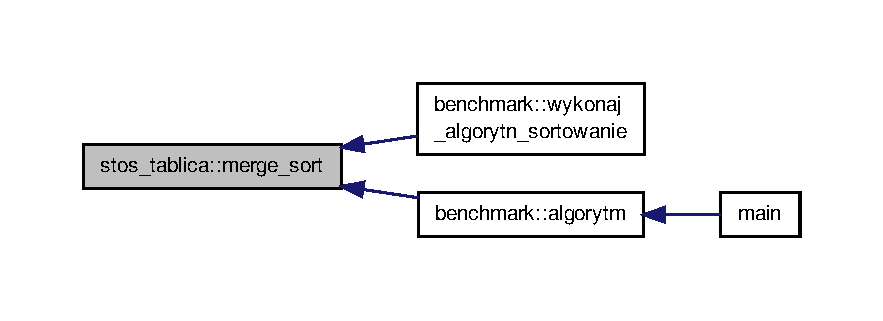
\includegraphics[width=350pt]{classstos__tablica_afaad303fc8eef3b5c115d5da31c38bc1_icgraph}
\end{center}
\end{figure}


\hypertarget{classstos__tablica_a79d983833ba1481654c51787bb604936}{\index{stos\-\_\-tablica@{stos\-\_\-tablica}!mergesort@{mergesort}}
\index{mergesort@{mergesort}!stos_tablica@{stos\-\_\-tablica}}
\subsubsection[{mergesort}]{\setlength{\rightskip}{0pt plus 5cm}void stos\-\_\-tablica\-::mergesort (
\begin{DoxyParamCaption}
\item[{int}]{pocz, }
\item[{int}]{kon}
\end{DoxyParamCaption}
)}}\label{classstos__tablica_a79d983833ba1481654c51787bb604936}


Funkcja sortujaca. 

Funkcja sortuje dane za pomoca algorytmu Merge Sort


\begin{DoxyParams}{Parameters}
{\em pocz} & -\/$>$ Pole typu int, zawiera informacje indeksie poczatkowym sortowanego zbioru\par
 \\
\hline
{\em kon} & -\/$>$ Pole typu int, zawiera informacje indeksie koncowym sortowanego zbioru \\
\hline
\end{DoxyParams}


Definition at line 160 of file stos\-\_\-tablica.\-cpp.

\hypertarget{classstos__tablica_a89f6cd04da8bafdded7b8d0f003e3978}{\index{stos\-\_\-tablica@{stos\-\_\-tablica}!pokaz\-\_\-elementy@{pokaz\-\_\-elementy}}
\index{pokaz\-\_\-elementy@{pokaz\-\_\-elementy}!stos_tablica@{stos\-\_\-tablica}}
\subsubsection[{pokaz\-\_\-elementy}]{\setlength{\rightskip}{0pt plus 5cm}void stos\-\_\-tablica\-::pokaz\-\_\-elementy (
\begin{DoxyParamCaption}
{}
\end{DoxyParamCaption}
)}}\label{classstos__tablica_a89f6cd04da8bafdded7b8d0f003e3978}


Funkcja wyswietlajaca. 

Funkcja wyswietla aktualny stan stosu 

Definition at line 7 of file stos\-\_\-tablica.\-cpp.

\hypertarget{classstos__tablica_aac88873e08b12ea26661690feb28ea86}{\index{stos\-\_\-tablica@{stos\-\_\-tablica}!przypisz@{przypisz}}
\index{przypisz@{przypisz}!stos_tablica@{stos\-\_\-tablica}}
\subsubsection[{przypisz}]{\setlength{\rightskip}{0pt plus 5cm}void stos\-\_\-tablica\-::przypisz (
\begin{DoxyParamCaption}
{}
\end{DoxyParamCaption}
)}}\label{classstos__tablica_aac88873e08b12ea26661690feb28ea86}


Funkcja przypisujaca. 

Funkcja przypisuje wartosci dynamicznej, pomocniczej tabeli danetmp do tabeli glownej programu -\/$>$ dane 

Definition at line 64 of file stos\-\_\-tablica.\-cpp.



Here is the caller graph for this function\-:
\nopagebreak
\begin{figure}[H]
\begin{center}
\leavevmode
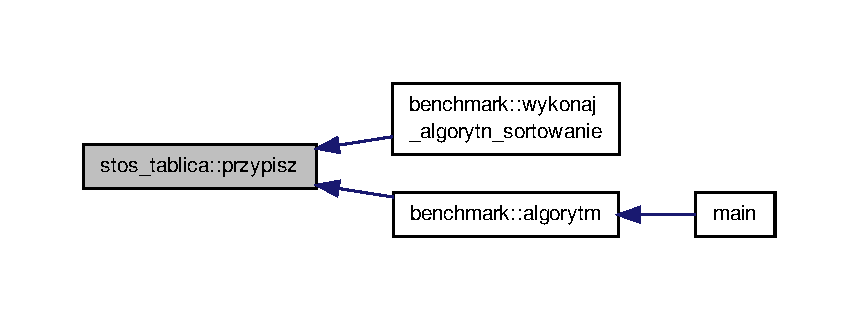
\includegraphics[width=350pt]{classstos__tablica_aac88873e08b12ea26661690feb28ea86_icgraph}
\end{center}
\end{figure}


\hypertarget{classstos__tablica_a636f59632a29c985a404c0c8a3a9a18f}{\index{stos\-\_\-tablica@{stos\-\_\-tablica}!quick\-\_\-sort@{quick\-\_\-sort}}
\index{quick\-\_\-sort@{quick\-\_\-sort}!stos_tablica@{stos\-\_\-tablica}}
\subsubsection[{quick\-\_\-sort}]{\setlength{\rightskip}{0pt plus 5cm}void stos\-\_\-tablica\-::quick\-\_\-sort (
\begin{DoxyParamCaption}
{}
\end{DoxyParamCaption}
)\hspace{0.3cm}{\ttfamily [inline]}}}\label{classstos__tablica_a636f59632a29c985a404c0c8a3a9a18f}


Funkcja wywolujaca funkcje sorujaca Quick Sort. 

Funkcja jest tylko po to, aby mozna bylo w kklasie innej niz ta uruchomic funkcje sortowania bezparametrycznie 

Definition at line 145 of file stos\-\_\-tablica.\-hh.



Here is the caller graph for this function\-:
\nopagebreak
\begin{figure}[H]
\begin{center}
\leavevmode
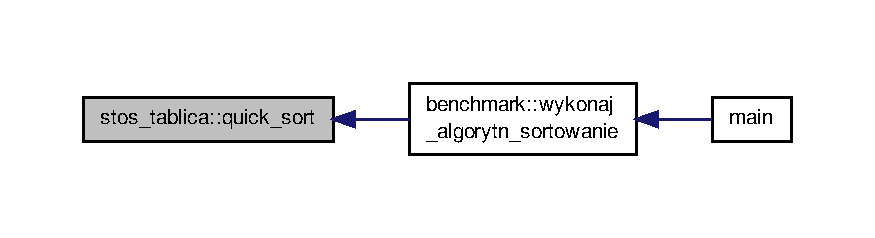
\includegraphics[width=350pt]{classstos__tablica_a636f59632a29c985a404c0c8a3a9a18f_icgraph}
\end{center}
\end{figure}


\hypertarget{classstos__tablica_a340038b0ac6af3983de3fe21fa54aa36}{\index{stos\-\_\-tablica@{stos\-\_\-tablica}!quicksort@{quicksort}}
\index{quicksort@{quicksort}!stos_tablica@{stos\-\_\-tablica}}
\subsubsection[{quicksort}]{\setlength{\rightskip}{0pt plus 5cm}void stos\-\_\-tablica\-::quicksort (
\begin{DoxyParamCaption}
\item[{int}]{left, }
\item[{int}]{right}
\end{DoxyParamCaption}
)}}\label{classstos__tablica_a340038b0ac6af3983de3fe21fa54aa36}


Funkcja sortujaca. 

Funkcja sortuje dane za pomoca algorytmu Quick Sort


\begin{DoxyParams}{Parameters}
{\em left} & -\/$>$ Pole typu int, zawiera informacje indeksie poczatkowym sortowanego zbioru\par
 \\
\hline
{\em right} & -\/$>$ Pole typu int, zawiera informacje indeksie koncowym sortowanego zbioru \\
\hline
\end{DoxyParams}


Definition at line 126 of file stos\-\_\-tablica.\-cpp.

\hypertarget{classstos__tablica_a64e273a78434133331b24a4f9bbff87b}{\index{stos\-\_\-tablica@{stos\-\_\-tablica}!swap@{swap}}
\index{swap@{swap}!stos_tablica@{stos\-\_\-tablica}}
\subsubsection[{swap}]{\setlength{\rightskip}{0pt plus 5cm}void stos\-\_\-tablica\-::swap (
\begin{DoxyParamCaption}
\item[{int $\ast$}]{x, }
\item[{int $\ast$}]{y}
\end{DoxyParamCaption}
)}}\label{classstos__tablica_a64e273a78434133331b24a4f9bbff87b}


Funkcja zamieniania wartosci. 

Funkcja zamienia wartosciami obiekty, ktore sa argumentami funkcji 
\begin{DoxyParams}{Parameters}
{\em x} & -\/$>$ Pole typu $\ast$int, zawiera adres obiektu, ktorego wartosc ma byc zamieniona z obiektem y\par
 \\
\hline
{\em y} & -\/$>$ Pole typu $\ast$int, zawiera adres obiektu, ktorego wartosc ma byc zamieniona z obiektem x \\
\hline
\end{DoxyParams}


Definition at line 153 of file stos\-\_\-tablica.\-cpp.

\hypertarget{classstos__tablica_a68d7d3ed8622663ff7aca3b9696724c5}{\index{stos\-\_\-tablica@{stos\-\_\-tablica}!wczytaj\-\_\-dane@{wczytaj\-\_\-dane}}
\index{wczytaj\-\_\-dane@{wczytaj\-\_\-dane}!stos_tablica@{stos\-\_\-tablica}}
\subsubsection[{wczytaj\-\_\-dane}]{\setlength{\rightskip}{0pt plus 5cm}void stos\-\_\-tablica\-::wczytaj\-\_\-dane (
\begin{DoxyParamCaption}
{}
\end{DoxyParamCaption}
)}}\label{classstos__tablica_a68d7d3ed8622663ff7aca3b9696724c5}


Funkcja wczytywania. 

Funkcja wczytuje wartosci do tabeli z podanego pliku przez uzytkownika. 

Definition at line 19 of file stos\-\_\-tablica.\-cpp.



Here is the caller graph for this function\-:
\nopagebreak
\begin{figure}[H]
\begin{center}
\leavevmode
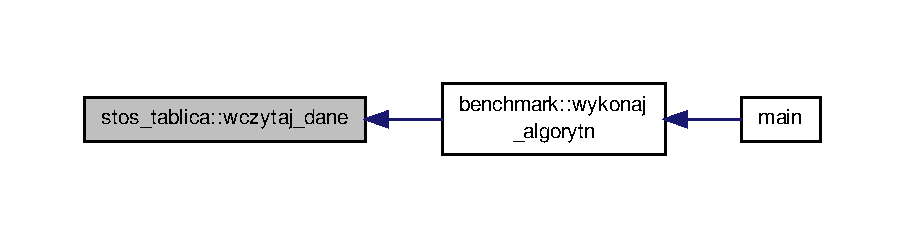
\includegraphics[width=350pt]{classstos__tablica_a68d7d3ed8622663ff7aca3b9696724c5_icgraph}
\end{center}
\end{figure}


\hypertarget{classstos__tablica_a33b9257de4213c84e96e666898f5ead0}{\index{stos\-\_\-tablica@{stos\-\_\-tablica}!wczytaj\-\_\-dane@{wczytaj\-\_\-dane}}
\index{wczytaj\-\_\-dane@{wczytaj\-\_\-dane}!stos_tablica@{stos\-\_\-tablica}}
\subsubsection[{wczytaj\-\_\-dane}]{\setlength{\rightskip}{0pt plus 5cm}void stos\-\_\-tablica\-::wczytaj\-\_\-dane (
\begin{DoxyParamCaption}
\item[{string}]{nazwa}
\end{DoxyParamCaption}
)}}\label{classstos__tablica_a33b9257de4213c84e96e666898f5ead0}


Funkcja wczytywania. 

Funkcja wczytuje wartosci do tabeli po przez wpisanie nazwy jako argument metody Wykorzystuje metode push jako funkcje wpisujaca do stosu


\begin{DoxyParams}{Parameters}
{\em nazwa} & -\/$>$ zmienna typu string, przechowuje nazwe otwieranego pliku \\
\hline
\end{DoxyParams}


Definition at line 43 of file stos\-\_\-tablica.\-cpp.

\hypertarget{classstos__tablica_abeeb3fc4e2bc9a9b9917b3e996eb388e}{\index{stos\-\_\-tablica@{stos\-\_\-tablica}!wypelnij\-\_\-losowo@{wypelnij\-\_\-losowo}}
\index{wypelnij\-\_\-losowo@{wypelnij\-\_\-losowo}!stos_tablica@{stos\-\_\-tablica}}
\subsubsection[{wypelnij\-\_\-losowo}]{\setlength{\rightskip}{0pt plus 5cm}void stos\-\_\-tablica\-::wypelnij\-\_\-losowo (
\begin{DoxyParamCaption}
{}
\end{DoxyParamCaption}
)}}\label{classstos__tablica_abeeb3fc4e2bc9a9b9917b3e996eb388e}


Funkcja wypelniajaca stos losowymi wartosciami. 

Funkcja wypelnia stos losowymi wartosciami. Uzytkownik wybiera sam ile elementow ma zostac wpisanych 

Definition at line 79 of file stos\-\_\-tablica.\-cpp.

\hypertarget{classstos__tablica_a430a06f13dc5a74bca50b07cc993196c}{\index{stos\-\_\-tablica@{stos\-\_\-tablica}!wyzeruj\-\_\-stos@{wyzeruj\-\_\-stos}}
\index{wyzeruj\-\_\-stos@{wyzeruj\-\_\-stos}!stos_tablica@{stos\-\_\-tablica}}
\subsubsection[{wyzeruj\-\_\-stos}]{\setlength{\rightskip}{0pt plus 5cm}void stos\-\_\-tablica\-::wyzeruj\-\_\-stos (
\begin{DoxyParamCaption}
{}
\end{DoxyParamCaption}
)}}\label{classstos__tablica_a430a06f13dc5a74bca50b07cc993196c}


Funkcja zerujaca stos. 

Funkcja kasuje dynamicznie zaalokowana tablice dane, zeby mozna bylo wpisac kolejna tablice z tymi samymi wartosciami Dodatkowo zeruje pola klasy zwiazane z ową tablica 

Definition at line 99 of file stos\-\_\-tablica.\-cpp.

\hypertarget{classstos__tablica_aabebf0add57a2440cddd9b4305d165f8}{\index{stos\-\_\-tablica@{stos\-\_\-tablica}!wyzeruj\-\_\-stos\-\_\-caly@{wyzeruj\-\_\-stos\-\_\-caly}}
\index{wyzeruj\-\_\-stos\-\_\-caly@{wyzeruj\-\_\-stos\-\_\-caly}!stos_tablica@{stos\-\_\-tablica}}
\subsubsection[{wyzeruj\-\_\-stos\-\_\-caly}]{\setlength{\rightskip}{0pt plus 5cm}void stos\-\_\-tablica\-::wyzeruj\-\_\-stos\-\_\-caly (
\begin{DoxyParamCaption}
{}
\end{DoxyParamCaption}
)}}\label{classstos__tablica_aabebf0add57a2440cddd9b4305d165f8}


Funkcja zerujaca caly stos. 

Funkcja kasuje wszystkie dynamicznie zaalokowane obiekty. Dodatkowo zeruje wszystkie pola klasy \hyperlink{classstos__tablica}{stos\-\_\-tablica} 

Definition at line 110 of file stos\-\_\-tablica.\-cpp.



Here is the caller graph for this function\-:
\nopagebreak
\begin{figure}[H]
\begin{center}
\leavevmode
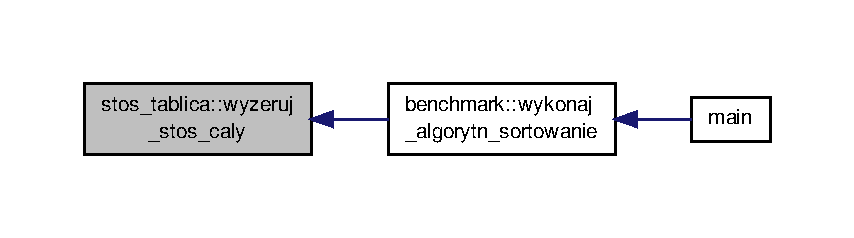
\includegraphics[width=350pt]{classstos__tablica_aabebf0add57a2440cddd9b4305d165f8_icgraph}
\end{center}
\end{figure}




\subsection{Member Data Documentation}
\hypertarget{classstos__tablica_a008b0f69384d5d987782c2f24fcbd387}{\index{stos\-\_\-tablica@{stos\-\_\-tablica}!dane@{dane}}
\index{dane@{dane}!stos_tablica@{stos\-\_\-tablica}}
\subsubsection[{dane}]{\setlength{\rightskip}{0pt plus 5cm}int$\ast$ stos\-\_\-tablica\-::dane\hspace{0.3cm}{\ttfamily [private]}}}\label{classstos__tablica_a008b0f69384d5d987782c2f24fcbd387}


Pole typu int, bedzie uzywane jako stosu z danymi. 



Definition at line 38 of file stos\-\_\-tablica.\-hh.

\hypertarget{classstos__tablica_a2ee83414df31c2f56383199a5d47c755}{\index{stos\-\_\-tablica@{stos\-\_\-tablica}!danetmp@{danetmp}}
\index{danetmp@{danetmp}!stos_tablica@{stos\-\_\-tablica}}
\subsubsection[{danetmp}]{\setlength{\rightskip}{0pt plus 5cm}int$\ast$ stos\-\_\-tablica\-::danetmp\hspace{0.3cm}{\ttfamily [private]}}}\label{classstos__tablica_a2ee83414df31c2f56383199a5d47c755}


Pole typu int, bedzie uzywane jako stosu z danymi sprawdzajacymi, pomocniczymi. 



Definition at line 42 of file stos\-\_\-tablica.\-hh.

\hypertarget{classstos__tablica_ae1737beb175c9041e44ff8b374fa3565}{\index{stos\-\_\-tablica@{stos\-\_\-tablica}!heap\-\_\-size@{heap\-\_\-size}}
\index{heap\-\_\-size@{heap\-\_\-size}!stos_tablica@{stos\-\_\-tablica}}
\subsubsection[{heap\-\_\-size}]{\setlength{\rightskip}{0pt plus 5cm}int stos\-\_\-tablica\-::heap\-\_\-size\hspace{0.3cm}{\ttfamily [private]}}}\label{classstos__tablica_ae1737beb175c9041e44ff8b374fa3565}


Pole typu int, bedzie uzywane jako pomocnicza wartosc do metody Heap Size. 



Definition at line 62 of file stos\-\_\-tablica.\-hh.

\hypertarget{classstos__tablica_addee4392050e497f2b9f07a5e7a17606}{\index{stos\-\_\-tablica@{stos\-\_\-tablica}!lewy@{lewy}}
\index{lewy@{lewy}!stos_tablica@{stos\-\_\-tablica}}
\subsubsection[{lewy}]{\setlength{\rightskip}{0pt plus 5cm}int stos\-\_\-tablica\-::lewy\hspace{0.3cm}{\ttfamily [private]}}}\label{classstos__tablica_addee4392050e497f2b9f07a5e7a17606}


Pole typu int, bedzie uzywane jako pomocnicza wartosc do metody Quick Sort. 



Definition at line 54 of file stos\-\_\-tablica.\-hh.

\hypertarget{classstos__tablica_aab32beac5ab0f185fb27492736798749}{\index{stos\-\_\-tablica@{stos\-\_\-tablica}!prawy@{prawy}}
\index{prawy@{prawy}!stos_tablica@{stos\-\_\-tablica}}
\subsubsection[{prawy}]{\setlength{\rightskip}{0pt plus 5cm}int stos\-\_\-tablica\-::prawy\hspace{0.3cm}{\ttfamily [private]}}}\label{classstos__tablica_aab32beac5ab0f185fb27492736798749}


Pole typu int, bedzie uzywane jako pomocnicza wartosc do metody Quick Sort. 



Definition at line 58 of file stos\-\_\-tablica.\-hh.

\hypertarget{classstos__tablica_aa9c1d33bd477174602d2632c74ebea9c}{\index{stos\-\_\-tablica@{stos\-\_\-tablica}!rozmiar@{rozmiar}}
\index{rozmiar@{rozmiar}!stos_tablica@{stos\-\_\-tablica}}
\subsubsection[{rozmiar}]{\setlength{\rightskip}{0pt plus 5cm}int stos\-\_\-tablica\-::rozmiar\hspace{0.3cm}{\ttfamily [private]}}}\label{classstos__tablica_aa9c1d33bd477174602d2632c74ebea9c}


Pole typu int, bedzie uzywane jako rozmiar tabeli. 



Definition at line 46 of file stos\-\_\-tablica.\-hh.

\hypertarget{classstos__tablica_adcfe2091d485a93da47eb9fb6a337b06}{\index{stos\-\_\-tablica@{stos\-\_\-tablica}!rozmiar\-\_\-tmp@{rozmiar\-\_\-tmp}}
\index{rozmiar\-\_\-tmp@{rozmiar\-\_\-tmp}!stos_tablica@{stos\-\_\-tablica}}
\subsubsection[{rozmiar\-\_\-tmp}]{\setlength{\rightskip}{0pt plus 5cm}int stos\-\_\-tablica\-::rozmiar\-\_\-tmp\hspace{0.3cm}{\ttfamily [private]}}}\label{classstos__tablica_adcfe2091d485a93da47eb9fb6a337b06}


Pole typu int, bedzie uzywane jako pomocnicza wartosc jako rozmiar stosu. 



Definition at line 50 of file stos\-\_\-tablica.\-hh.



The documentation for this class was generated from the following files\-:\begin{DoxyCompactItemize}
\item 
/home/pawel/\-Dokumenty/programowanie/pamsi/sortowanie/prj/inc/\hyperlink{stos__tablica_8hh}{stos\-\_\-tablica.\-hh}\item 
/home/pawel/\-Dokumenty/programowanie/pamsi/sortowanie/prj/src/\hyperlink{stos__tablica_8cpp}{stos\-\_\-tablica.\-cpp}\end{DoxyCompactItemize}

\chapter{File Documentation}
\hypertarget{strona_8dox}{\section{/home/pawel/\-Dokumenty/programowanie/pamsi/sortowanie/prj/doc/pages/strona.dox File Reference}
\label{strona_8dox}\index{/home/pawel/\-Dokumenty/programowanie/pamsi/sortowanie/prj/doc/pages/strona.\-dox@{/home/pawel/\-Dokumenty/programowanie/pamsi/sortowanie/prj/doc/pages/strona.\-dox}}
}

\hypertarget{benchmark_8hh}{\section{/home/pawel/\-Dokumenty/programowanie/pamsi/zad3/prj/inc/benchmark.hh File Reference}
\label{benchmark_8hh}\index{/home/pawel/\-Dokumenty/programowanie/pamsi/zad3/prj/inc/benchmark.\-hh@{/home/pawel/\-Dokumenty/programowanie/pamsi/zad3/prj/inc/benchmark.\-hh}}
}


Definicje funkcji dla klasy benchmark.  


{\ttfamily \#include $<$fstream$>$}\\*
{\ttfamily \#include $<$iostream$>$}\\*
{\ttfamily \#include $<$math.\-h$>$}\\*
{\ttfamily \#include $<$string.\-h$>$}\\*
{\ttfamily \#include $<$stdio.\-h$>$}\\*
{\ttfamily \#include $<$sys/time.\-h$>$}\\*
{\ttfamily \#include \char`\"{}kolejka\-\_\-tablica.\-hh\char`\"{}}\\*
{\ttfamily \#include \char`\"{}kolejka\-\_\-lista.\-hh\char`\"{}}\\*
{\ttfamily \#include \char`\"{}stos\-\_\-tablica.\-hh\char`\"{}}\\*
{\ttfamily \#include \char`\"{}stos\-\_\-lista.\-hh\char`\"{}}\\*
Include dependency graph for benchmark.\-hh\-:\nopagebreak
\begin{figure}[H]
\begin{center}
\leavevmode
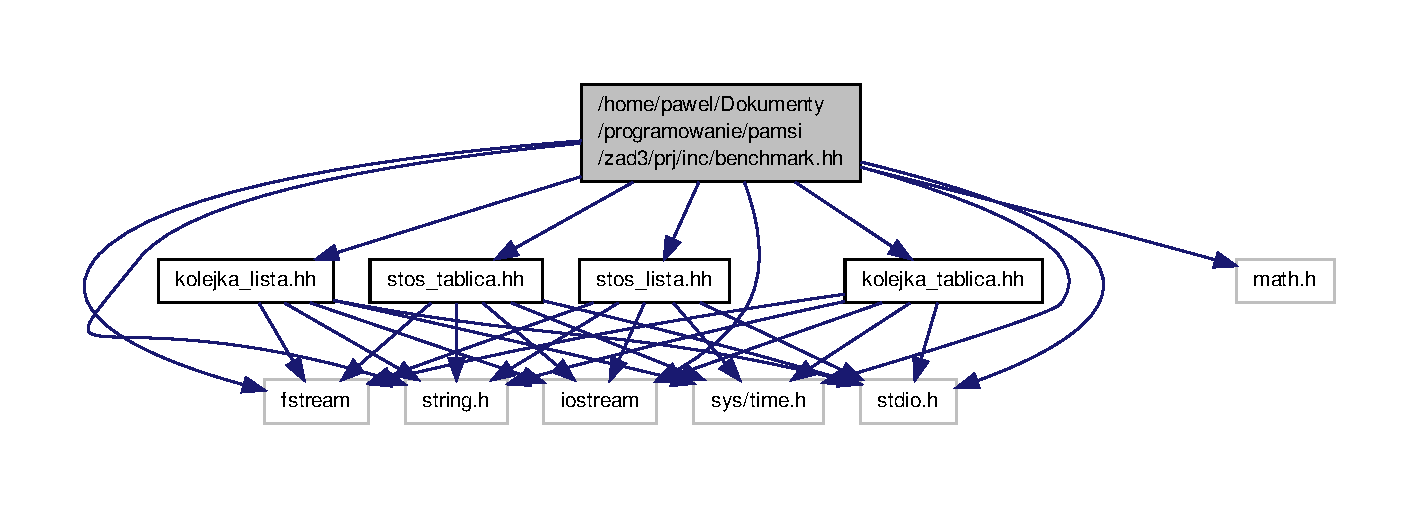
\includegraphics[width=350pt]{benchmark_8hh__incl}
\end{center}
\end{figure}
This graph shows which files directly or indirectly include this file\-:\nopagebreak
\begin{figure}[H]
\begin{center}
\leavevmode
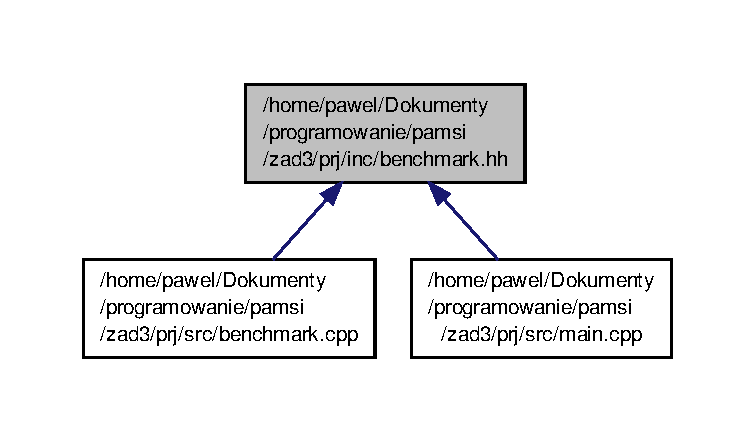
\includegraphics[width=350pt]{benchmark_8hh__dep__incl}
\end{center}
\end{figure}
\subsection*{Classes}
\begin{DoxyCompactItemize}
\item 
class \hyperlink{classbenchmark}{benchmark}
\begin{DoxyCompactList}\small\item\em Modeluje pojecie Benchmark. \end{DoxyCompactList}\end{DoxyCompactItemize}


\subsection{Detailed Description}
Definicje funkcji dla klasy benchmark. 

Definition in file \hyperlink{benchmark_8hh_source}{benchmark.\-hh}.


\hypertarget{kolejka__lista_8hh}{\section{/home/pawel/\-Dokumenty/programowanie/pamsi/zad3/prj/inc/kolejka\-\_\-lista.hh File Reference}
\label{kolejka__lista_8hh}\index{/home/pawel/\-Dokumenty/programowanie/pamsi/zad3/prj/inc/kolejka\-\_\-lista.\-hh@{/home/pawel/\-Dokumenty/programowanie/pamsi/zad3/prj/inc/kolejka\-\_\-lista.\-hh}}
}


Definicje funkcji dla klasy Kolejka zdefiniowanej lista.  


{\ttfamily \#include $<$fstream$>$}\\*
{\ttfamily \#include $<$iostream$>$}\\*
{\ttfamily \#include $<$string.\-h$>$}\\*
{\ttfamily \#include $<$stdio.\-h$>$}\\*
{\ttfamily \#include $<$sys/time.\-h$>$}\\*
Include dependency graph for kolejka\-\_\-lista.\-hh\-:\nopagebreak
\begin{figure}[H]
\begin{center}
\leavevmode
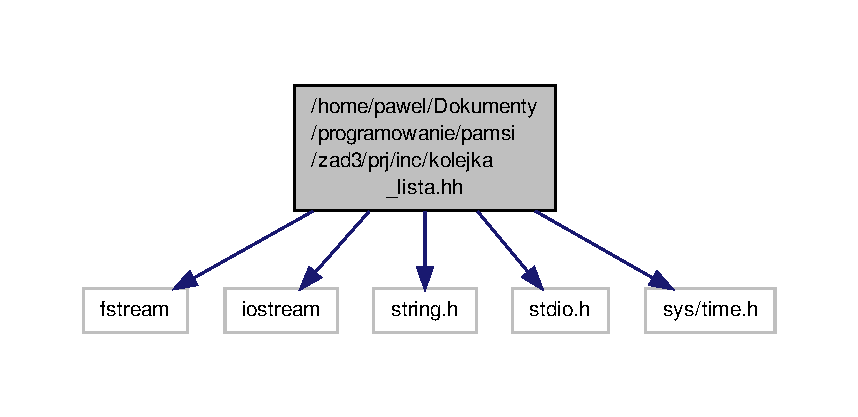
\includegraphics[width=350pt]{kolejka__lista_8hh__incl}
\end{center}
\end{figure}
This graph shows which files directly or indirectly include this file\-:\nopagebreak
\begin{figure}[H]
\begin{center}
\leavevmode
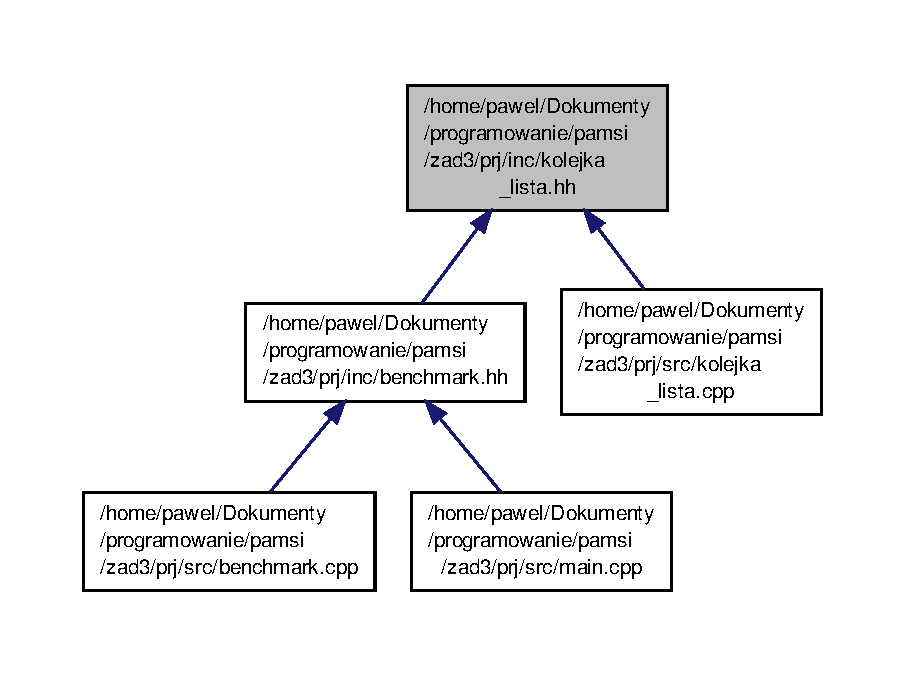
\includegraphics[width=350pt]{kolejka__lista_8hh__dep__incl}
\end{center}
\end{figure}
\subsection*{Classes}
\begin{DoxyCompactItemize}
\item 
class \hyperlink{classelementk}{elementk}
\begin{DoxyCompactList}\small\item\em Modeluje pojecie elementk (zmieniona nazwa, poniewaz \hyperlink{classstos__lista}{stos\-\_\-lista} tez ma klase o nazwie element). \end{DoxyCompactList}\item 
class \hyperlink{classkolejka__lista}{kolejka\-\_\-lista}
\begin{DoxyCompactList}\small\item\em Modeluje pojecie Kolejka. \end{DoxyCompactList}\end{DoxyCompactItemize}


\subsection{Detailed Description}
Definicje funkcji dla klasy Kolejka zdefiniowanej lista. 

Definition in file \hyperlink{kolejka__lista_8hh_source}{kolejka\-\_\-lista.\-hh}.


\hypertarget{kolejka__tablica_8hh}{\section{/home/pawel/\-Dokumenty/programowanie/pamsi/zad3/prj/inc/kolejka\-\_\-tablica.hh File Reference}
\label{kolejka__tablica_8hh}\index{/home/pawel/\-Dokumenty/programowanie/pamsi/zad3/prj/inc/kolejka\-\_\-tablica.\-hh@{/home/pawel/\-Dokumenty/programowanie/pamsi/zad3/prj/inc/kolejka\-\_\-tablica.\-hh}}
}


Definicje funkcji dla klasy Kolejka zdefiniowanej tablica.  


{\ttfamily \#include $<$fstream$>$}\\*
{\ttfamily \#include $<$iostream$>$}\\*
{\ttfamily \#include $<$string.\-h$>$}\\*
{\ttfamily \#include $<$stdio.\-h$>$}\\*
{\ttfamily \#include $<$sys/time.\-h$>$}\\*
Include dependency graph for kolejka\-\_\-tablica.\-hh\-:\nopagebreak
\begin{figure}[H]
\begin{center}
\leavevmode
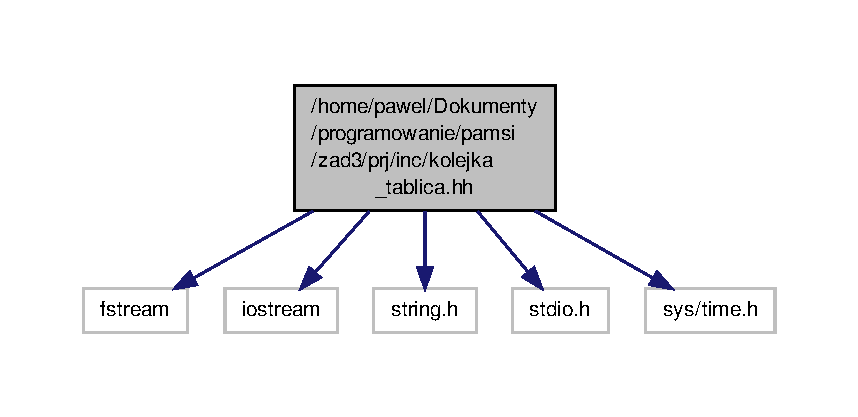
\includegraphics[width=350pt]{kolejka__tablica_8hh__incl}
\end{center}
\end{figure}
This graph shows which files directly or indirectly include this file\-:\nopagebreak
\begin{figure}[H]
\begin{center}
\leavevmode
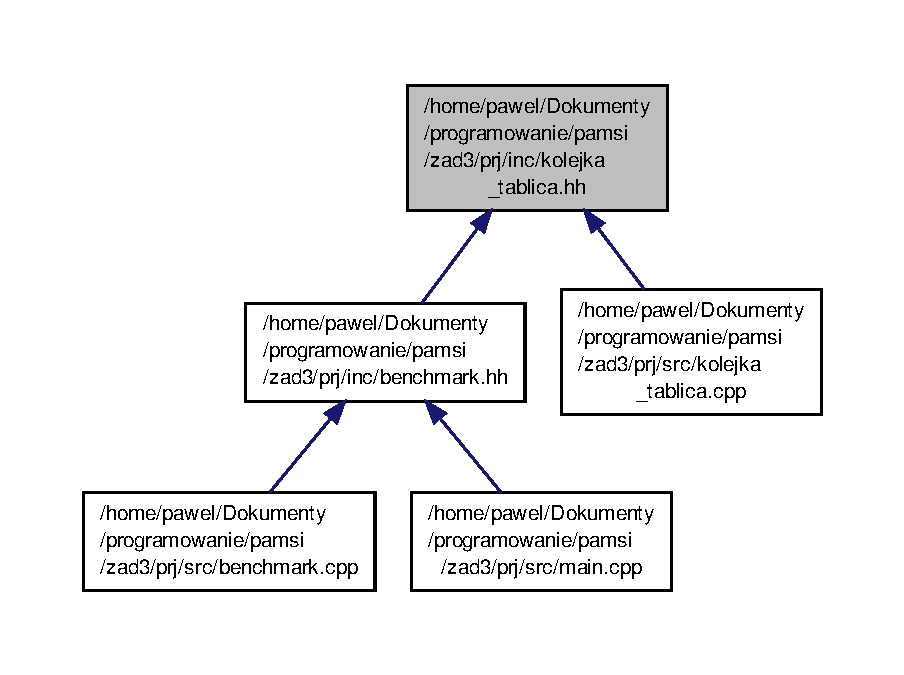
\includegraphics[width=350pt]{kolejka__tablica_8hh__dep__incl}
\end{center}
\end{figure}
\subsection*{Classes}
\begin{DoxyCompactItemize}
\item 
class \hyperlink{classkolejka__tablica}{kolejka\-\_\-tablica}
\begin{DoxyCompactList}\small\item\em Modeluje pojecie Kolejka. \end{DoxyCompactList}\end{DoxyCompactItemize}


\subsection{Detailed Description}
Definicje funkcji dla klasy Kolejka zdefiniowanej tablica. 

Definition in file \hyperlink{kolejka__tablica_8hh_source}{kolejka\-\_\-tablica.\-hh}.


\hypertarget{stos__lista_8hh}{\section{/home/pawel/\-Dokumenty/programowanie/pamsi/zad3/prj/inc/stos\-\_\-lista.hh File Reference}
\label{stos__lista_8hh}\index{/home/pawel/\-Dokumenty/programowanie/pamsi/zad3/prj/inc/stos\-\_\-lista.\-hh@{/home/pawel/\-Dokumenty/programowanie/pamsi/zad3/prj/inc/stos\-\_\-lista.\-hh}}
}


Definicje funkcji dla klasy Stos zdefiniowanej lista.  


{\ttfamily \#include $<$fstream$>$}\\*
{\ttfamily \#include $<$iostream$>$}\\*
{\ttfamily \#include $<$string.\-h$>$}\\*
{\ttfamily \#include $<$stdio.\-h$>$}\\*
{\ttfamily \#include $<$sys/time.\-h$>$}\\*
Include dependency graph for stos\-\_\-lista.\-hh\-:\nopagebreak
\begin{figure}[H]
\begin{center}
\leavevmode
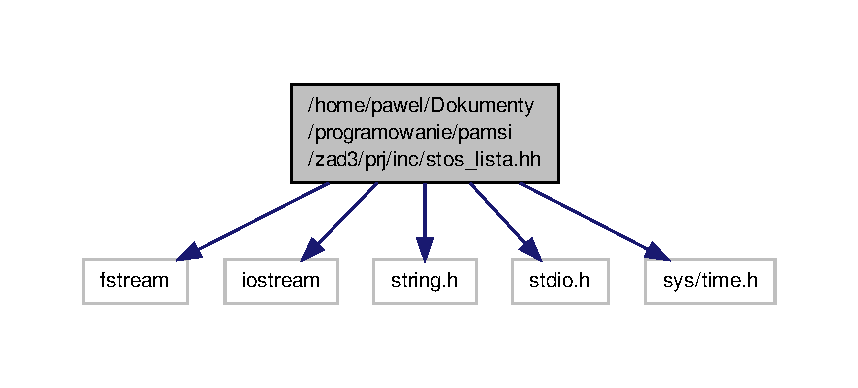
\includegraphics[width=350pt]{stos__lista_8hh__incl}
\end{center}
\end{figure}
This graph shows which files directly or indirectly include this file\-:\nopagebreak
\begin{figure}[H]
\begin{center}
\leavevmode
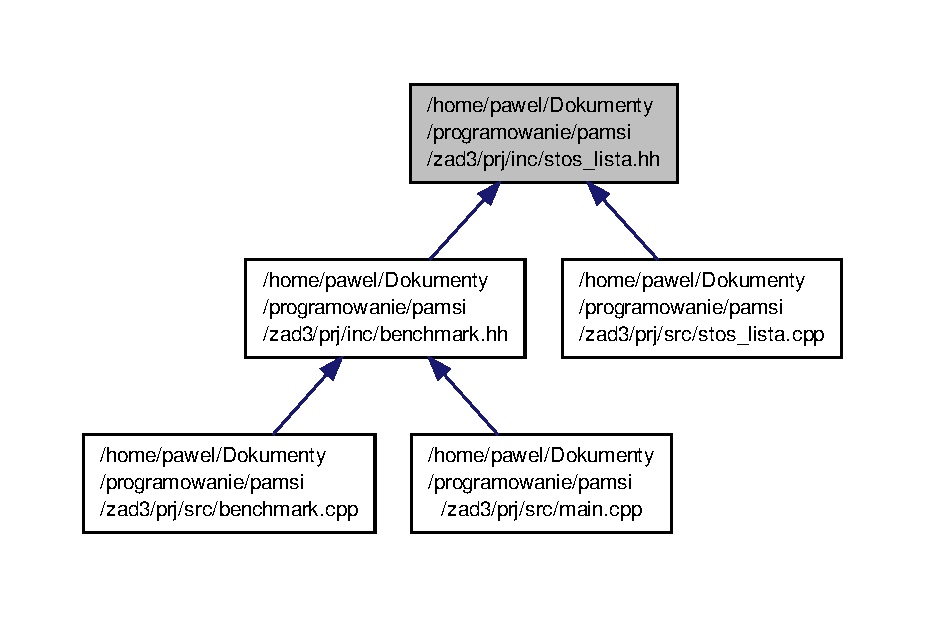
\includegraphics[width=350pt]{stos__lista_8hh__dep__incl}
\end{center}
\end{figure}
\subsection*{Classes}
\begin{DoxyCompactItemize}
\item 
class \hyperlink{classelement}{element}
\begin{DoxyCompactList}\small\item\em Modeluje pojecie element. \end{DoxyCompactList}\item 
class \hyperlink{classstos__lista}{stos\-\_\-lista}
\begin{DoxyCompactList}\small\item\em Modeluje pojecie Stos. \end{DoxyCompactList}\end{DoxyCompactItemize}


\subsection{Detailed Description}
Definicje funkcji dla klasy Stos zdefiniowanej lista. 

Definition in file \hyperlink{stos__lista_8hh_source}{stos\-\_\-lista.\-hh}.


\hypertarget{stos__tablica_8hh}{\section{/home/pawel/\-Dokumenty/programowanie/pamsi/sortowaniev2/prj/inc/stos\-\_\-tablica.hh File Reference}
\label{stos__tablica_8hh}\index{/home/pawel/\-Dokumenty/programowanie/pamsi/sortowaniev2/prj/inc/stos\-\_\-tablica.\-hh@{/home/pawel/\-Dokumenty/programowanie/pamsi/sortowaniev2/prj/inc/stos\-\_\-tablica.\-hh}}
}


Definicje funkcji dla klasy Stos zdefiniowanej tablica.  


{\ttfamily \#include $<$fstream$>$}\\*
{\ttfamily \#include $<$iostream$>$}\\*
{\ttfamily \#include $<$string.\-h$>$}\\*
{\ttfamily \#include $<$stdio.\-h$>$}\\*
{\ttfamily \#include $<$cstdlib$>$}\\*
{\ttfamily \#include $<$sys/time.\-h$>$}\\*
{\ttfamily \#include $<$cmath$>$}\\*
{\ttfamily \#include \char`\"{}stdlib.\-h\char`\"{}}\\*
{\ttfamily \#include \char`\"{}time.\-h\char`\"{}}\\*
Include dependency graph for stos\-\_\-tablica.\-hh\-:\nopagebreak
\begin{figure}[H]
\begin{center}
\leavevmode
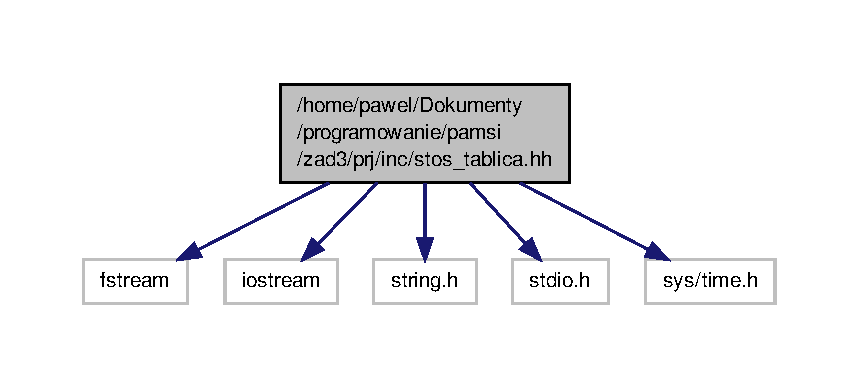
\includegraphics[width=350pt]{stos__tablica_8hh__incl}
\end{center}
\end{figure}
This graph shows which files directly or indirectly include this file\-:\nopagebreak
\begin{figure}[H]
\begin{center}
\leavevmode
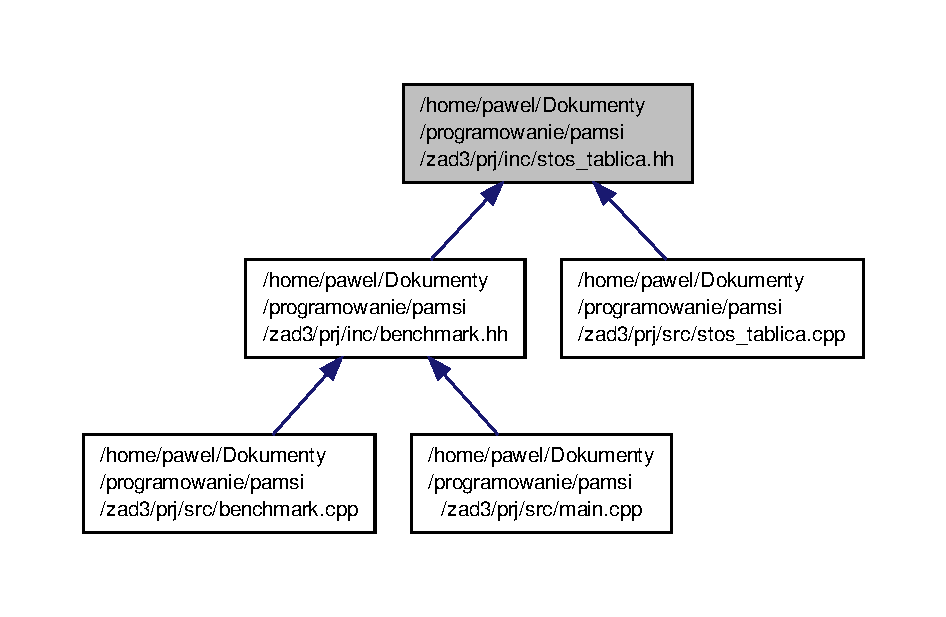
\includegraphics[width=350pt]{stos__tablica_8hh__dep__incl}
\end{center}
\end{figure}
\subsection*{Classes}
\begin{DoxyCompactItemize}
\item 
class \hyperlink{classstos__tablica}{stos\-\_\-tablica}
\begin{DoxyCompactList}\small\item\em Modeluje pojecie Stos. \end{DoxyCompactList}\end{DoxyCompactItemize}


\subsection{Detailed Description}
Definicje funkcji dla klasy Stos zdefiniowanej tablica. 

Definition in file \hyperlink{stos__tablica_8hh_source}{stos\-\_\-tablica.\-hh}.


\hypertarget{benchmark_8cpp}{\section{/home/pawel/\-Dokumenty/programowanie/pamsi/sortowaniev2/prj/src/benchmark.cpp File Reference}
\label{benchmark_8cpp}\index{/home/pawel/\-Dokumenty/programowanie/pamsi/sortowaniev2/prj/src/benchmark.\-cpp@{/home/pawel/\-Dokumenty/programowanie/pamsi/sortowaniev2/prj/src/benchmark.\-cpp}}
}


Plik zawiera funkcje z klasy benchmark.  


{\ttfamily \#include \char`\"{}../inc/benchmark.\-hh\char`\"{}}\\*
{\ttfamily \#include $<$iostream$>$}\\*
Include dependency graph for benchmark.\-cpp\-:\nopagebreak
\begin{figure}[H]
\begin{center}
\leavevmode
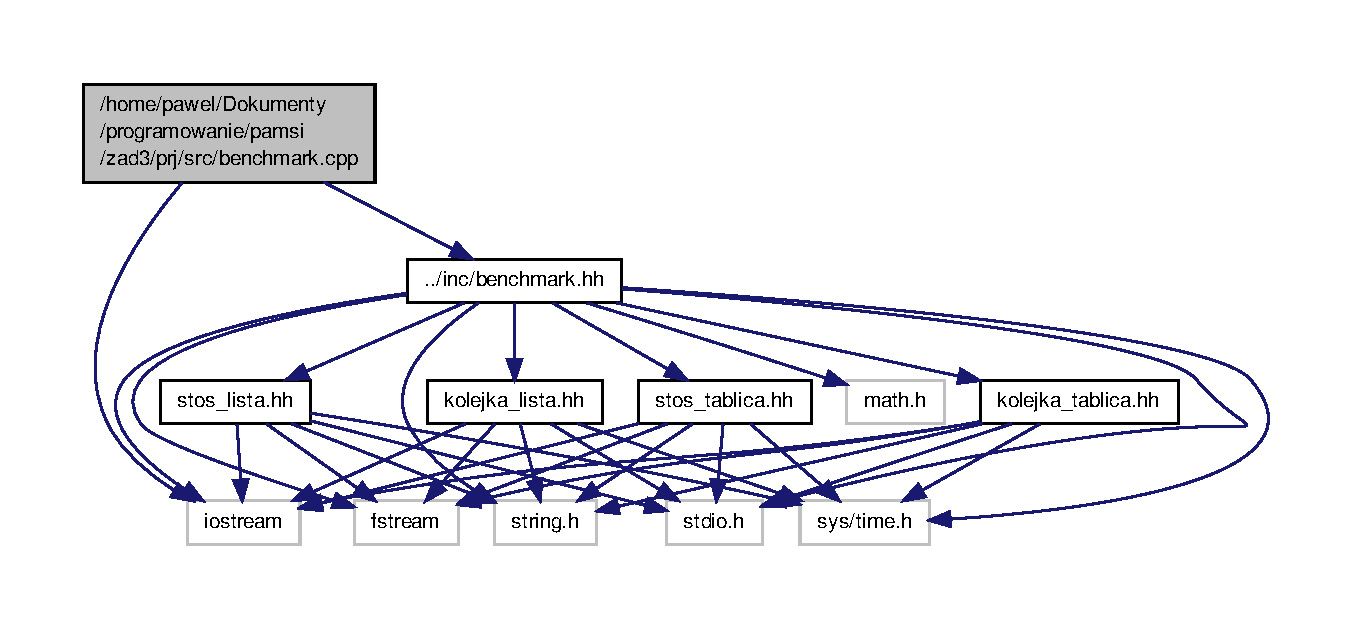
\includegraphics[width=350pt]{benchmark_8cpp__incl}
\end{center}
\end{figure}


\subsection{Detailed Description}
Plik zawiera funkcje z klasy benchmark. 

Definition in file \hyperlink{benchmark_8cpp_source}{benchmark.\-cpp}.


\hypertarget{kolejka__lista_8cpp}{\section{/home/pawel/\-Dokumenty/programowanie/pamsi/zad3/prj/src/kolejka\-\_\-lista.cpp File Reference}
\label{kolejka__lista_8cpp}\index{/home/pawel/\-Dokumenty/programowanie/pamsi/zad3/prj/src/kolejka\-\_\-lista.\-cpp@{/home/pawel/\-Dokumenty/programowanie/pamsi/zad3/prj/src/kolejka\-\_\-lista.\-cpp}}
}
{\ttfamily \#include \char`\"{}../inc/kolejka\-\_\-lista.\-hh\char`\"{}}\\*
{\ttfamily \#include $<$iostream$>$}\\*
Include dependency graph for kolejka\-\_\-lista.\-cpp\-:\nopagebreak
\begin{figure}[H]
\begin{center}
\leavevmode
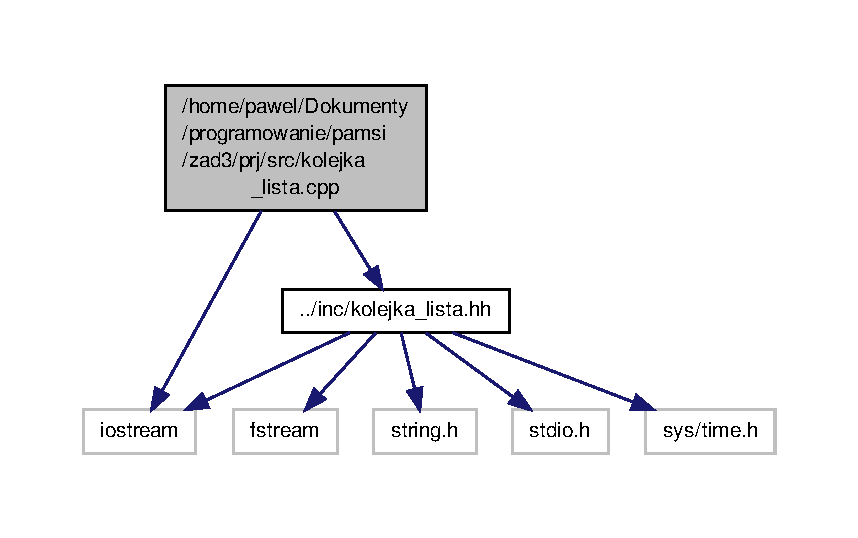
\includegraphics[width=350pt]{kolejka__lista_8cpp__incl}
\end{center}
\end{figure}

\hypertarget{kolejka__tablica_8cpp}{\section{/home/pawel/\-Dokumenty/programowanie/pamsi/zad3/prj/src/kolejka\-\_\-tablica.cpp File Reference}
\label{kolejka__tablica_8cpp}\index{/home/pawel/\-Dokumenty/programowanie/pamsi/zad3/prj/src/kolejka\-\_\-tablica.\-cpp@{/home/pawel/\-Dokumenty/programowanie/pamsi/zad3/prj/src/kolejka\-\_\-tablica.\-cpp}}
}
{\ttfamily \#include \char`\"{}../inc/kolejka\-\_\-tablica.\-hh\char`\"{}}\\*
Include dependency graph for kolejka\-\_\-tablica.\-cpp\-:\nopagebreak
\begin{figure}[H]
\begin{center}
\leavevmode
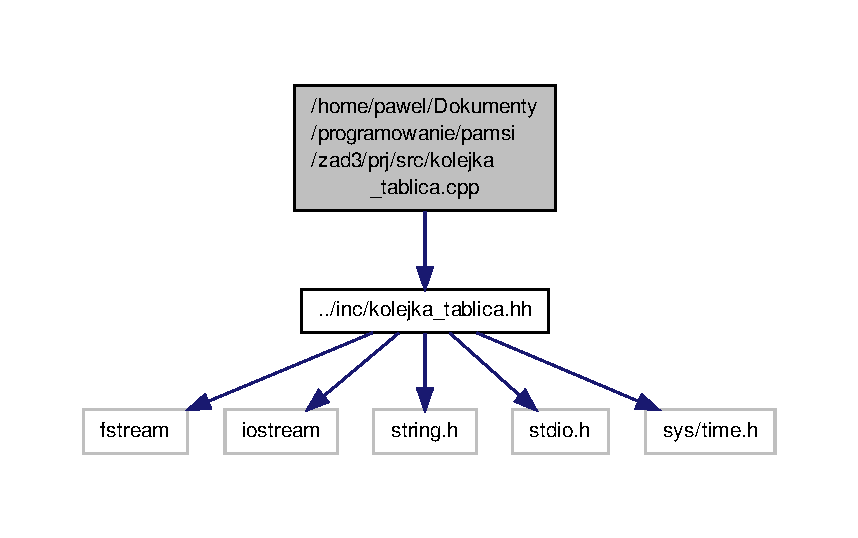
\includegraphics[width=350pt]{kolejka__tablica_8cpp__incl}
\end{center}
\end{figure}

\hypertarget{main_8cpp}{\section{/home/pawel/\-Dokumenty/programowanie/pamsi/simplex/prj/src/main.cpp File Reference}
\label{main_8cpp}\index{/home/pawel/\-Dokumenty/programowanie/pamsi/simplex/prj/src/main.\-cpp@{/home/pawel/\-Dokumenty/programowanie/pamsi/simplex/prj/src/main.\-cpp}}
}


Plik zawiera funkcje \hyperlink{main_8cpp_ae66f6b31b5ad750f1fe042a706a4e3d4}{main()}  


{\ttfamily \#include $<$iostream$>$}\\*
{\ttfamily \#include \char`\"{}../inc/simplex.\-hh\char`\"{}}\\*
Include dependency graph for main.\-cpp\-:\nopagebreak
\begin{figure}[H]
\begin{center}
\leavevmode
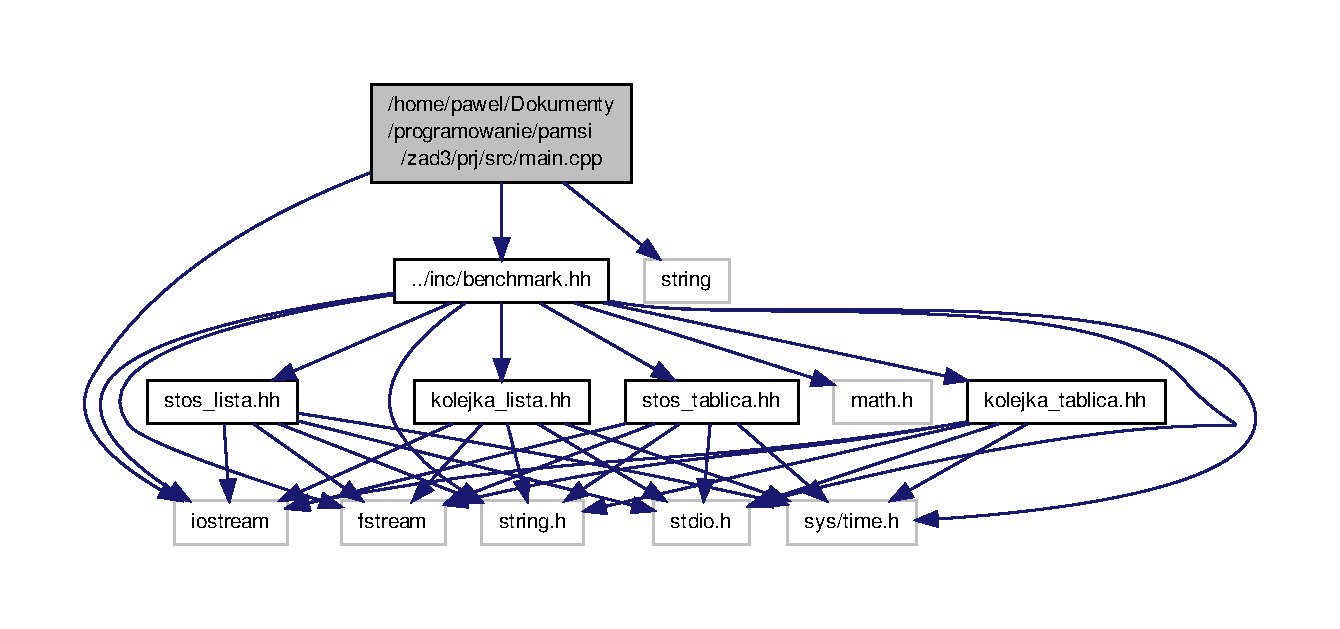
\includegraphics[width=224pt]{main_8cpp__incl}
\end{center}
\end{figure}
\subsection*{Functions}
\begin{DoxyCompactItemize}
\item 
int \hyperlink{main_8cpp_ae66f6b31b5ad750f1fe042a706a4e3d4}{main} ()
\end{DoxyCompactItemize}


\subsection{Detailed Description}
Plik zawiera funkcje \hyperlink{main_8cpp_ae66f6b31b5ad750f1fe042a706a4e3d4}{main()} 

Definition in file \hyperlink{main_8cpp_source}{main.\-cpp}.



\subsection{Function Documentation}
\hypertarget{main_8cpp_ae66f6b31b5ad750f1fe042a706a4e3d4}{\index{main.\-cpp@{main.\-cpp}!main@{main}}
\index{main@{main}!main.cpp@{main.\-cpp}}
\subsubsection[{main}]{\setlength{\rightskip}{0pt plus 5cm}int main (
\begin{DoxyParamCaption}
{}
\end{DoxyParamCaption}
)}}\label{main_8cpp_ae66f6b31b5ad750f1fe042a706a4e3d4}


Definition at line 13 of file main.\-cpp.



Here is the call graph for this function\-:\nopagebreak
\begin{figure}[H]
\begin{center}
\leavevmode
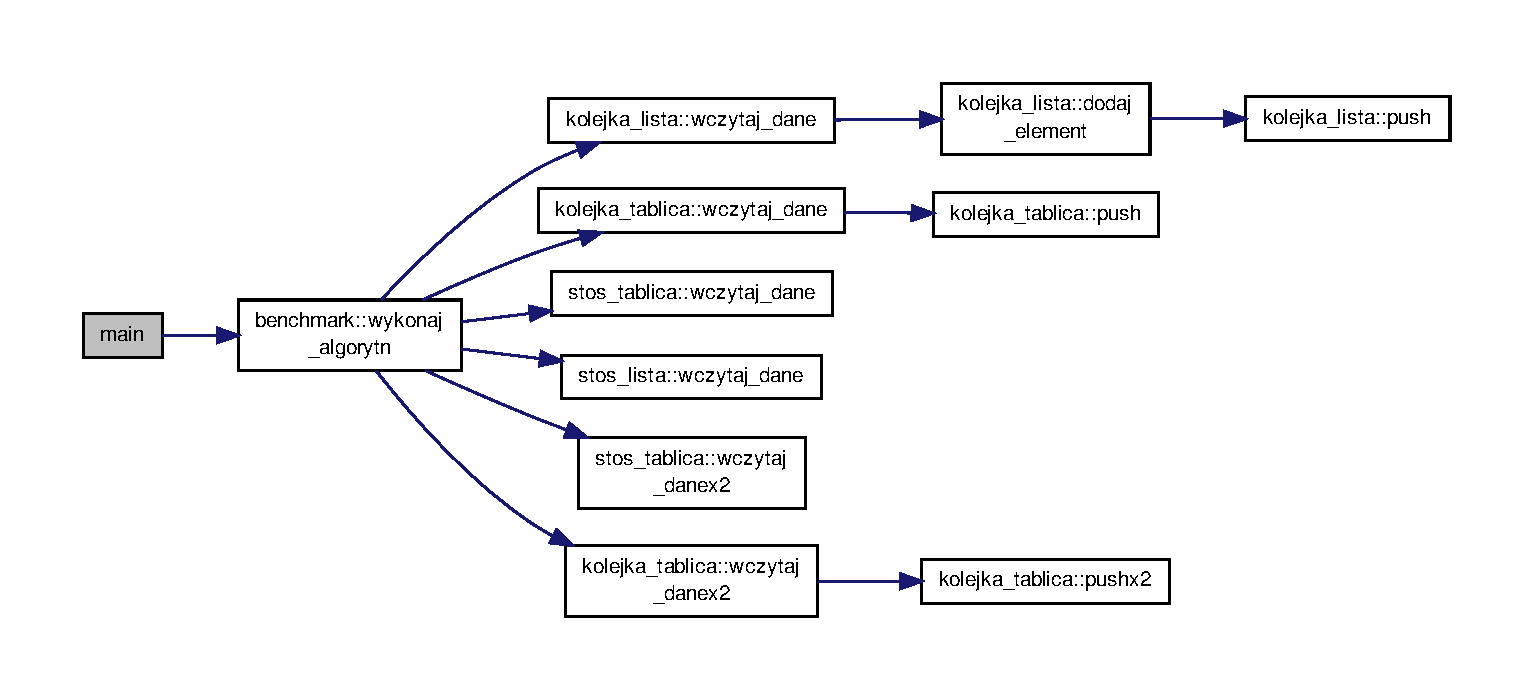
\includegraphics[width=282pt]{main_8cpp_ae66f6b31b5ad750f1fe042a706a4e3d4_cgraph}
\end{center}
\end{figure}



\hypertarget{stos__lista_8cpp}{\section{/home/pawel/\-Dokumenty/programowanie/pamsi/zad3/prj/src/stos\-\_\-lista.cpp File Reference}
\label{stos__lista_8cpp}\index{/home/pawel/\-Dokumenty/programowanie/pamsi/zad3/prj/src/stos\-\_\-lista.\-cpp@{/home/pawel/\-Dokumenty/programowanie/pamsi/zad3/prj/src/stos\-\_\-lista.\-cpp}}
}
{\ttfamily \#include \char`\"{}../inc/stos\-\_\-lista.\-hh\char`\"{}}\\*
{\ttfamily \#include $<$iostream$>$}\\*
Include dependency graph for stos\-\_\-lista.\-cpp\-:\nopagebreak
\begin{figure}[H]
\begin{center}
\leavevmode
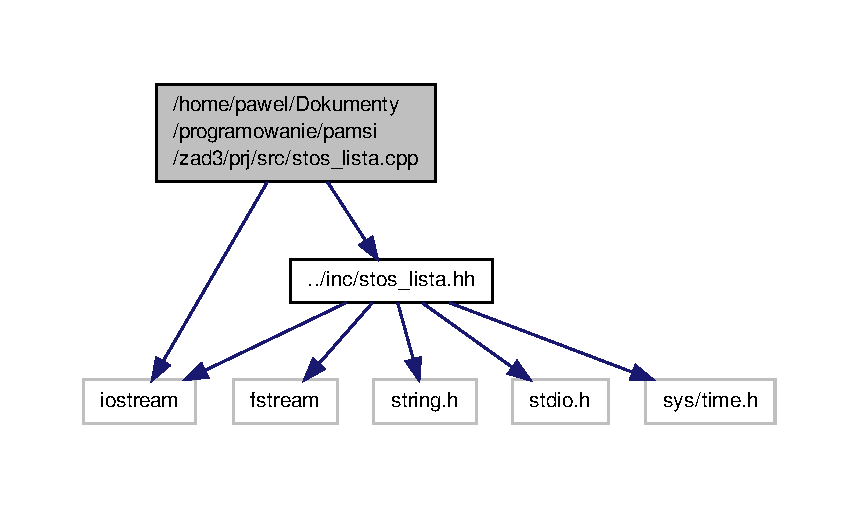
\includegraphics[width=350pt]{stos__lista_8cpp__incl}
\end{center}
\end{figure}

\hypertarget{stos__tablica_8cpp}{\section{/home/pawel/\-Dokumenty/programowanie/pamsi/zad3/prj/src/stos\-\_\-tablica.cpp File Reference}
\label{stos__tablica_8cpp}\index{/home/pawel/\-Dokumenty/programowanie/pamsi/zad3/prj/src/stos\-\_\-tablica.\-cpp@{/home/pawel/\-Dokumenty/programowanie/pamsi/zad3/prj/src/stos\-\_\-tablica.\-cpp}}
}
{\ttfamily \#include \char`\"{}../inc/stos\-\_\-tablica.\-hh\char`\"{}}\\*
{\ttfamily \#include $<$iostream$>$}\\*
Include dependency graph for stos\-\_\-tablica.\-cpp\-:\nopagebreak
\begin{figure}[H]
\begin{center}
\leavevmode
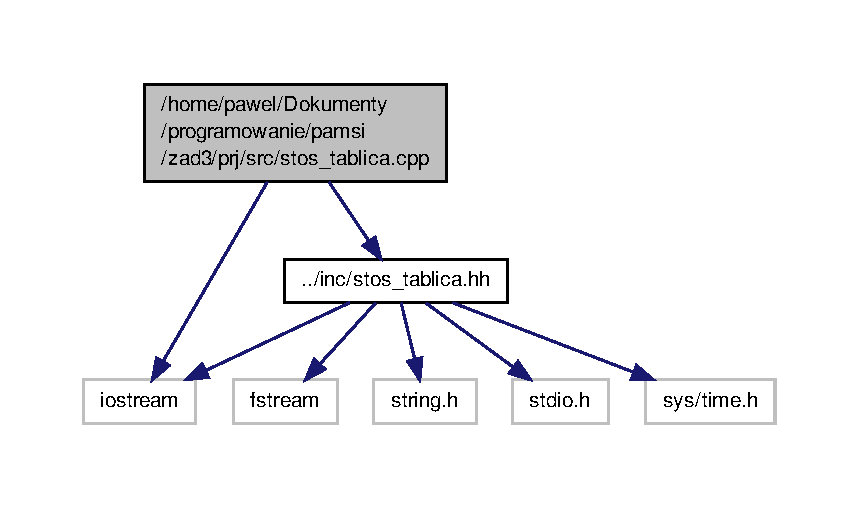
\includegraphics[width=350pt]{stos__tablica_8cpp__incl}
\end{center}
\end{figure}

%--- End generated contents ---

% Index
\newpage
\phantomsection
\addcontentsline{toc}{part}{Index}
\printindex

\end{document}
